%
% Tutorial -- Getting Started with Digital Circuit Simulation
%
% Copyright (C) 2006 Mike Brinson <mbrin72043@yahoo.co.uk>
%
% Permission is granted to copy, distribute and/or modify this document
% under the terms of the GNU Free Documentation License, Version 1.1
% or any later version published by the Free Software Foundation.
%

% redefine subfigure caption
\renewcommand{\thesubfigure}{\thefigure(\alph{subfigure})}
\makeatletter
  \renewcommand{\@thesubfigure}{\thesubfigure:\space}
  \renewcommand{\p@subfigure}{}
\makeatother

% redefine subtable caption
\renewcommand{\thesubtable}{\thetable(\alph{subtable})}
\makeatletter
  \renewcommand{\@thesubtable}{\thesubtable:\space}
  \renewcommand{\p@subtable}{}
\makeatother

\tutsection{Introduction}

On 21 January 2006 Qucs 0.0.8 was released by the Qucs development
team.  This is the first version of the package to include digital
circuit simulation based on VHDL.  FreeHDL\footnote{The FreeHDL
Project, \url{http://www.freehdl.seul.org/}. } being chosen as the
VHDL engine.  In the period following the release of Qucs 0.0.8 there
has been considerable activity centred around finding and correcting a
number of bugs in the Qucs digital simulation code.  Many of these
fixes are now included in the latest CVS code and will eventually form
part of the next Qucs release.  This tutorial note is an attempt on my
part to communicate to other Qucs users a number of background ideas
concerning the capabilities and limitations of the current state of
Qucs VHDL simulation.  Much of the information reported here was
assembled by the author while assisting Michael Margraf to test and
debug the VHDL code generated by Qucs.  In the future, if there is
enough interest in these notes, or indeed in Qucs VHDL simulation in
general, I will update them as the Qucs digital simulation features
are improved.

\addvspace{12pt}

Qucs digital simulation follows a complex set of steps that are mostly
transparent to the software user.  In step one, a schematic
representing a digital circuit under test is drawn.  This schematic
consists of an interconnected group of Qucs digital components, one or
more user defined digital subcircuits (if required), and a copy of the
digital simulation icon with the timing or truth table parameters set.
In step two, the information recorded on a circuit schematic is
converted into a text file containing VHDL statements. These describe
the circuit components, their connection, and a testbench for
simulating circuit performance.  Next, FreeHDL is launched by Qucs to
convert the VHDL code file into a C++ source program.  This is
compiled to form an executable machine code simulation of the original
circuit.  Finally, Qucs runs this program, collects signal data as
digital signal events take place and displays signal waveforms as a
function of time or digital data in a truth table format.

\addvspace{12pt}

The VHDL code generated by Qucs 0.0.8 is limited in its scope by the
following factors:
\begin{itemize}
\item
Digital gates are described by data flow concurrent statements.
\item
Flip-flops and the digital signal generator are described by process
statements.
\item
Component connection wires (signals) can only be of type bit as
defined in the standard VHDL library\footnote{Signal type bit only
defines logic signals '0' and '1'.  Care must be taken to ensure that
signal contention does not occur during simulation because the
resulting logic state cannot be modelled with type bit. Signal
contention can happen when two or more digital devices attempt to
drive the same wire with logic '0' and logic '1' signals at the same
time.  Moreover, it is not possible to simulate the performance of
tristate devices using VHDL signal type bit.}.
\item
Digital bus structures are not allowed in this release of the Qucs
package.
\item
Digital subcircuits can be drawn as schematics and associated with a
symbol in a similar fashion to analogue subcircuits.
\item
Digital subcircuit pins can have type in, out, inout or analog.  Qucs
treats pins of type analog the same as VHDL pin type inout.
\item
Once defined digital subcircuits may be placed and connected to other
components on schematics.
\item
Multiple copies of the same digital subcircuit are allowed on a single
schematic.
\item
Digital subcircuits may also be nested; nesting has been tested to a
depth of four.
\end{itemize}

\tutsection{Simulating simple digital circuits}

The most basic form of digital circuit that can be simulated is one
consisting entirely of Qucs predefined digital components drawn on a
schematic having only one level of design hierarchy.  The truth table
for a simple combinational circuit of this type is shown in
Table~\ref{tab:tab1}.

\begin{table}
\centering
% use packages: array
\begin{tabular}{llll}
A & B & C & F \\ 
0 & 0 & 0 & 0 \\ 
0 & 0 & 1 & 1 \\ 
0 & 1 & 0 & 1 \\ 
0 & 1 & 1 & 0 \\ 
1 & 0 & 0 & 0 \\ 
1 & 0 & 1 & 1 \\ 
1 & 1 & 0 & 1 \\ 
1 & 1 & 1 & 0
\end{tabular}
\caption{Truth table for a logic circuit with inputs A, B, C and output F.}
\label{tab:tab1}
\end{table}
%\FloatBarrier

\begin{flushleft}
Output F can be expressed in sum of products Boolean form as
\end{flushleft}
\begin{center}
\begin{large}

$F = \overline{A}.\overline{B}.C + \overline{A}.B.\overline{C}+A.\overline{B}.C+A.B.\overline{C}$\end{large}
\end{center}

\begin{flushleft}
On minimisation, using Boolean algebra or a Karnaugh map, output F becomes
\end{flushleft}
\begin{center}
\begin{large}$F=A.C+B.\overline{C}$\end{large}
\end{center}
The schematic for example 1 is illustrated in Fig.~\ref{fig:dtut1}.
This diagram was constructed using the same techniques employed for
drawing analogue schematics.


\tutsubsection{Notes on drawing digital schematics}
\begin{itemize}
\item
The only predefined Qucs components that can be used to draw a digital
circuit schematic are (1) the digital components listed in the digital
components icon window, (2) the ground symbol, and (3) the digital
simulation icon.
\item
A useful tip when drawing digital schematics is to adopt the matrix
approach shown in Fig.~\ref{fig:dtut1}. Input signals flow from top to
bottom of the schematic and output signals are positioned on the
right-hand side of a horizontal line. This makes checking the circuit
schematic for errors much easier than the case where diagrams have
wires connecting components in an unstructured way.
\item
Input and output wires (signals) should be given names consistant with
the circuit being simulated, A, B, C and F in Fig.~\ref{fig:dtut1}.
If the signal wires are not named by the user, Qucs will allocate them
different arbitrary names.  This can make identification and selection
of signals for display on an output waveform graph, and indeed
checking for errors in a large circuit, much more difficult than it
need be.
\item
Notice in Fig.~\ref{fig:dtut1} the international symbols for the logic
gates are shown on the schematic.
\end{itemize}

\begin{figure}[ht]
  \centering
  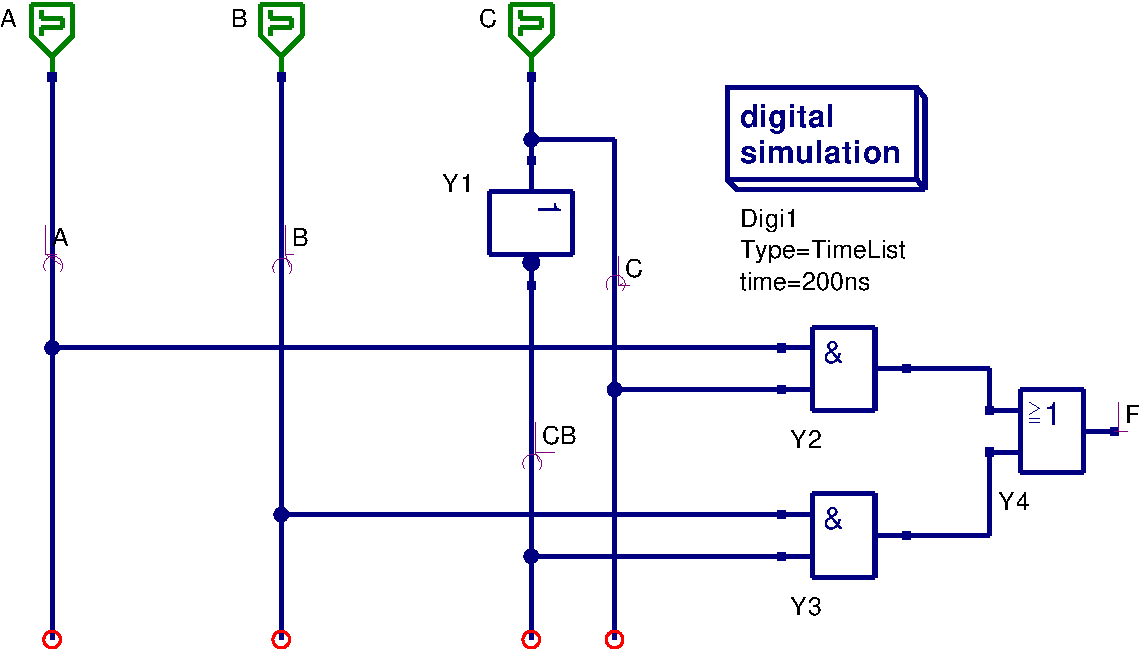
\includegraphics[width=0.9\linewidth]{dtut1}
  \caption{Qucs schematic for minimised logic function F.}
  \label{fig:dtut1}
\end{figure} 
%\FloatBarrier

\tutsection{VHDL code generated by Qucs}

Clicking the Qucs Simulate menu button (or pressing key F2) starts the
simulation process. At an early phase in this process Qucs writes a
text file to disk that contains the VHDL code for the circuit being
simulated.  This file can be displayed by clicking on the
\textit{\textbf{show last netlist}} drop down menu or by pressing key
F6. The VHDL code produced by Qucs for the circuit shown in
Fig.~\ref{fig:dtut1} is presented in Table~\ref{tab:tab2}.

\begin{table}
\begin{lstlisting}[
    language=VHDL,
    basicstyle=\small]
-- Qucs 0.0.9  tut1_ex1.sch
entity TestBench is
end entity;
use work.all;

architecture Arch_TestBench of TestBench is
signal CB, A,  B,  F, C, 
       nnnet0, 
       nnnet1 : bit;
begin
  nnnet0 <= C and A;
  nnnet1 <= CB and B;
  CB <= not C;

  A:process
  begin
    A <= '0';  wait for 40 ns;
    A <= '1';  wait for 40 ns;
  end process;


  B:process
  begin
    B <= '0';  wait for 20 ns;
    B <= '1';  wait for 20 ns;
  end process;

  F <= nnnet1 or nnnet0;

  C:process
  begin
    C <= '0';  wait for 10 ns;
    C <= '1';  wait for 10 ns;
  end process;

end architecture;
\end{lstlisting}
\caption{VHDL code for the circuit shown in Fig.~\ref{fig:dtut1}.}
\label{tab:tab2}
\end{table}
%\FloatBarrier

\addvspace{12pt}

Signals identified by nnnet0 and nnnet1 in Table~\ref{tab:tab2} have
been allocated these names by Qucs; nnnet0 and nnnet1 are internal
signal nets that are not named on the circuit schematic shown in
Fig.~\ref{fig:dtut1}.  Fig.~\ref{fig:tdex1} illustrates the starting
section of a typical Qucs digital functional waveform plot.  This
style of plot illustrates signal events without component delays.  If
required, signal delays can be specified for individual gates and
other components (from the component \textbf{\textit{edit properties}}
menu).  The VHDL code generated for components with delays will then
reflect such changes, for example adding a 10 ns delay to signal CB in
Table~\ref{tab:tab2} generates VHDL code
\begin{lstlisting}[language=VHDL]
CB <= not C after 10 ns;
\end{lstlisting}

Readers will probably have observed that the Qucs version number
referred to in Table~\ref{tab:tab2} VHDL listing is 0.0.9.  This is
the current CVS development version number.  Qucs 0.0.9 includes a
number of important bug fixes.  The remainder of these notes assume
readers have downloaded, and recompiled, the latest CVS code from
Sourceforge.net\footnote{Please note, Qucs Linux release 0.0.8 will
normally simulate single hierarchy digital circuits without error.
However, Qucs 0.0.8 does fail at the VHDL to C++ conversion phase if a
schematic includes more than one ground symbol.}.

\begin{figure}[ht]
  \centering
  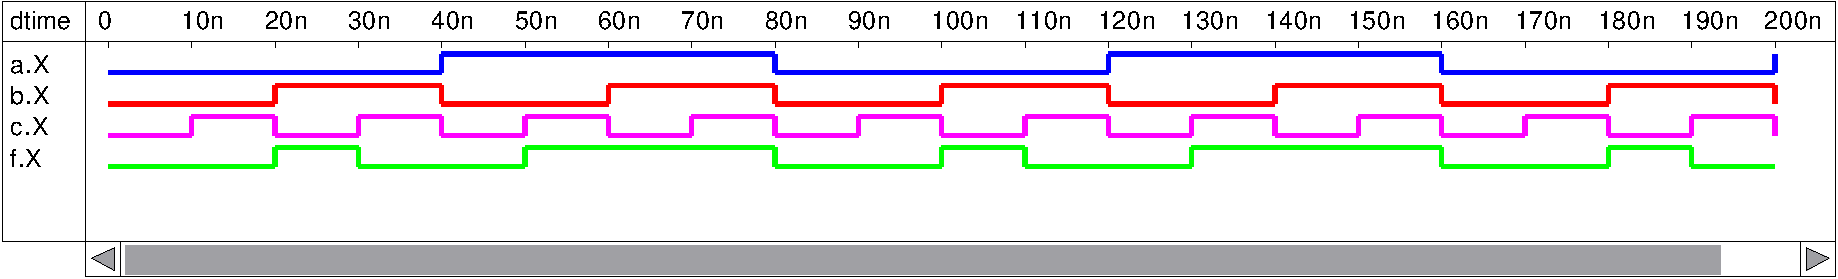
\includegraphics[width=1\linewidth]{tdex1}
  \caption{Digital functional waveforms for the circuit shown in Fig.~\ref{fig:dtut1}.}
  \label{fig:tdex1}
\end{figure}
\FloatBarrier

\tutsection{Truth tables}

Truth tables are one of the most fundamental and convenient ways of
displaying digital circuit data.  Qucs has a built-in facility that
allows a truth table to be generated from a schematic drawing.  This
feature is particularly useful when checking minimised logic designs
for errors.  Lets consider a simple but instructive example: A logic
circuit has four binary inputs A, B, C, and D, and one output P.
Output P is logic '1' when inputs ABCD are numbers in the decimal 
sequence 3, 5, 7, 11 and 13. In Boolean sum of product form

\begin{center}
\begin{large}$P=\overline{A}.\overline{B}.C.D+
\overline{A}.B.\overline{C}.D+\overline{A}.B.C.D+A.\overline{B}.C.D+
A.B.\overline{C}.D$
\end{large}\end{center}

This simplifies to
\begin{center}
\begin{large}$P=D.(A.B+B \oplus C )$\end{large}
\end{center}
The schematic for the sum of products equation for P is shown in
Fig.~\ref{fig:prim1sch}.  Similarly Fig.~\ref{fig:prim2sch} presents
the schematic for a minimised P equation.  Setting the digital
simulation type to TruthTable, rather than TimeList, causes Qucs on
pressing key F2, to generate a truth table based on the information
provided on a circuit schematic. The number of truth table inputs, and
indeed outputs, correspond to the number of input generators and the
number of named outputs. Truth tables for both schematics are given in
Table~\ref{tab:prim1tt} and~\ref{tab:prim2tt}. Comparing these two
tables clearly indicates that they are not identical and moreover
confirms that the minimised solution is not correct.  Reworking the
minimisation procedure points to the error being a missing signal
inversion.  The correct Boolean equation for P is

\begin{center}
\begin{large}$P=D.(\overline{A}.B+B \oplus C )$\end{large}
\end{center}

\begin{figure}
  \centering
\subfigure[Schematic diagram for sum of products equation P]{
  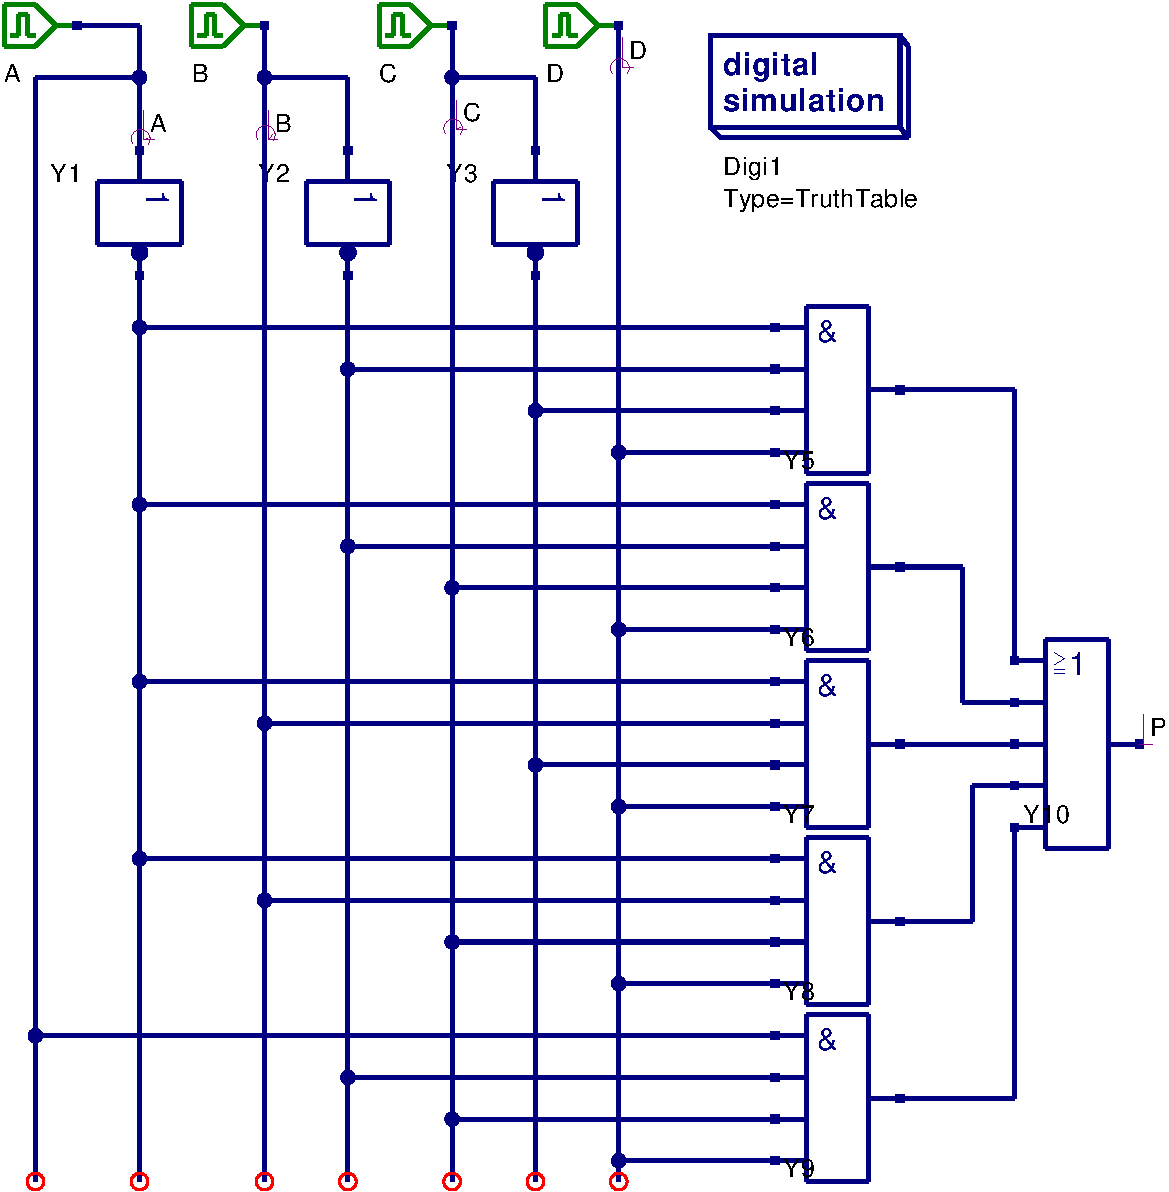
\includegraphics[width=.7\linewidth]{prim1sch}
  \label{fig:prim1sch}}
% prim1sch.png: 99.9998dpi, width=8.15cm, height=8.31cm, bb=0 0 321 327
\subfigure[Schematic diagram for minimised equation P]{
  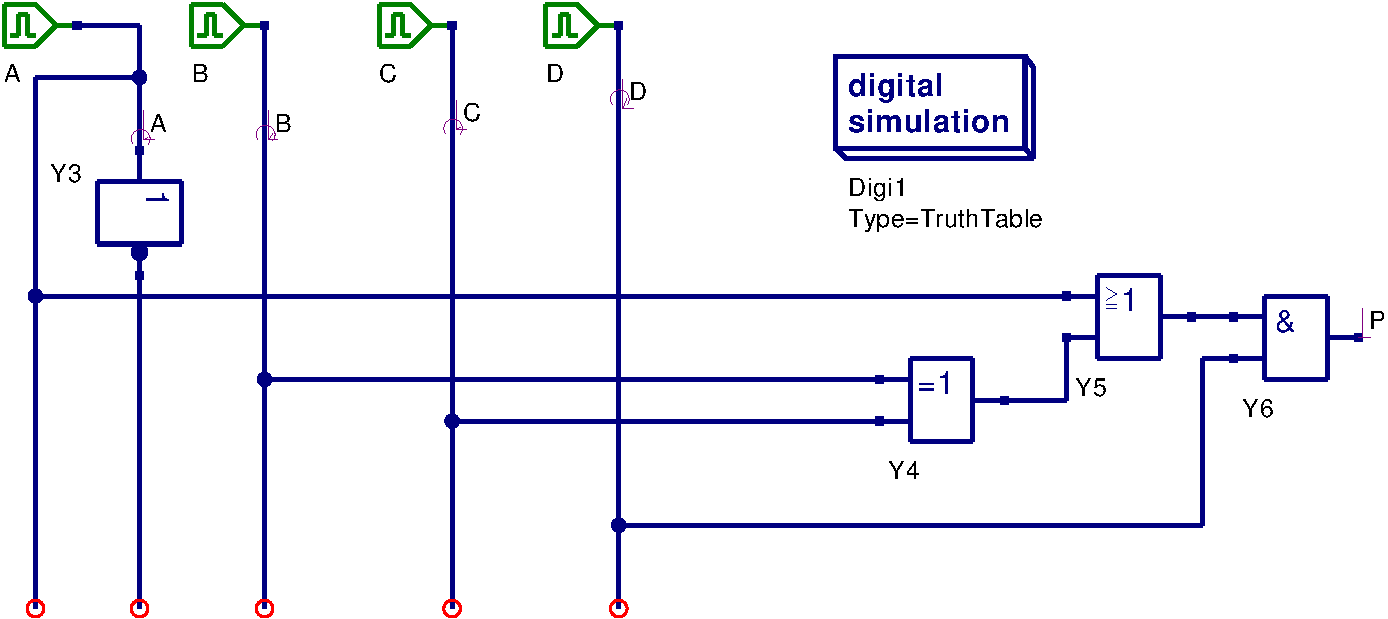
\includegraphics[width=.7\linewidth]{prim2sch}
  \label{fig:prim2sch}}
% prim1sch.png: 99.9998dpi, width=10.21cm, height=4.62cm, bb=0 0 402 182
\end{figure}
\FloatBarrier

\begin{table}
  \stepcounter{table}
  \centering
\subtable[Truth table for sum of products equation P]{
  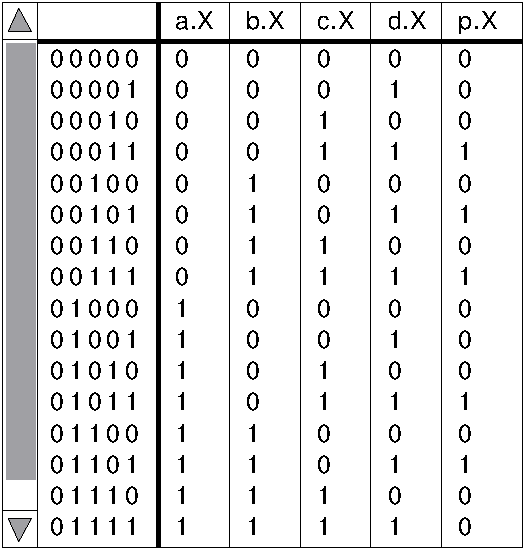
\includegraphics[width=.4\linewidth]{prim1tt}
% prim1tt.png: 200dpi, width=1.91cm, height=1.91cm, bb=0 0 150 150
  \label{tab:prim1tt}}
\\
\subtable[Truth table for minimised equation P]{
  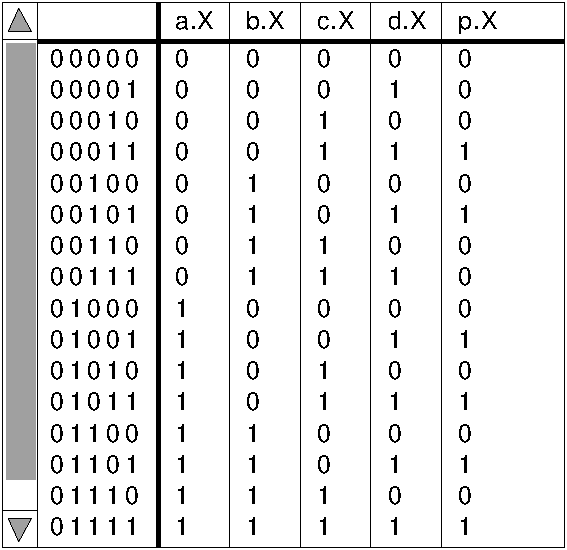
\includegraphics[width=.435\linewidth]{prim2tt}
  \label{tab:prim2tt}}
% prim2tt.png: 99.9998dpi, width=3.94cm, height=3.91cm, bb=0 0 155 154
\end{table}
\FloatBarrier

\tutsection{Digital subcircuits}

Although it is possible to draw complex schematic diagrams using only
the predefined digital components supplied with Qucs, this technique
can be extremely tedious, and is of course, prone to error.  When
drawing large schematics we require a design procedure that naturally
subdivides groups of digital components into self contained units.
These units can then be treated in the same way as basic digital
components when placing and connecting them on a schematic drawing.
In the world of analogue and digital circuit design such units are
often called subcircuits.\footnote{The circuit simulator SPICE is a
well known example of a widely used CAD program that makes extensive
use of subcircuits in circuit design.}  A subcircuit is defined by
three major attributes plus a number of other properties. The major
attributes are, firstly a digital circuit that defines circuit
function, secondly a circuit symbol that depicts a circuit in a higher
level of a design hierarchy, and thirdly the subcircuit input/output
pins shown on the subcircuit symbol.  Other properties include for
example, signal path delays. The process for generating digital
subcircuits is identical to that used for analogue subcircuits.  It is
best demonstrated by considering an example.
Figure~\ref{fig:t1ex2sch} shows the schematic for a four input
combinational circuit.

\begin{figure}
  \stepcounter{figure}
  \centering
  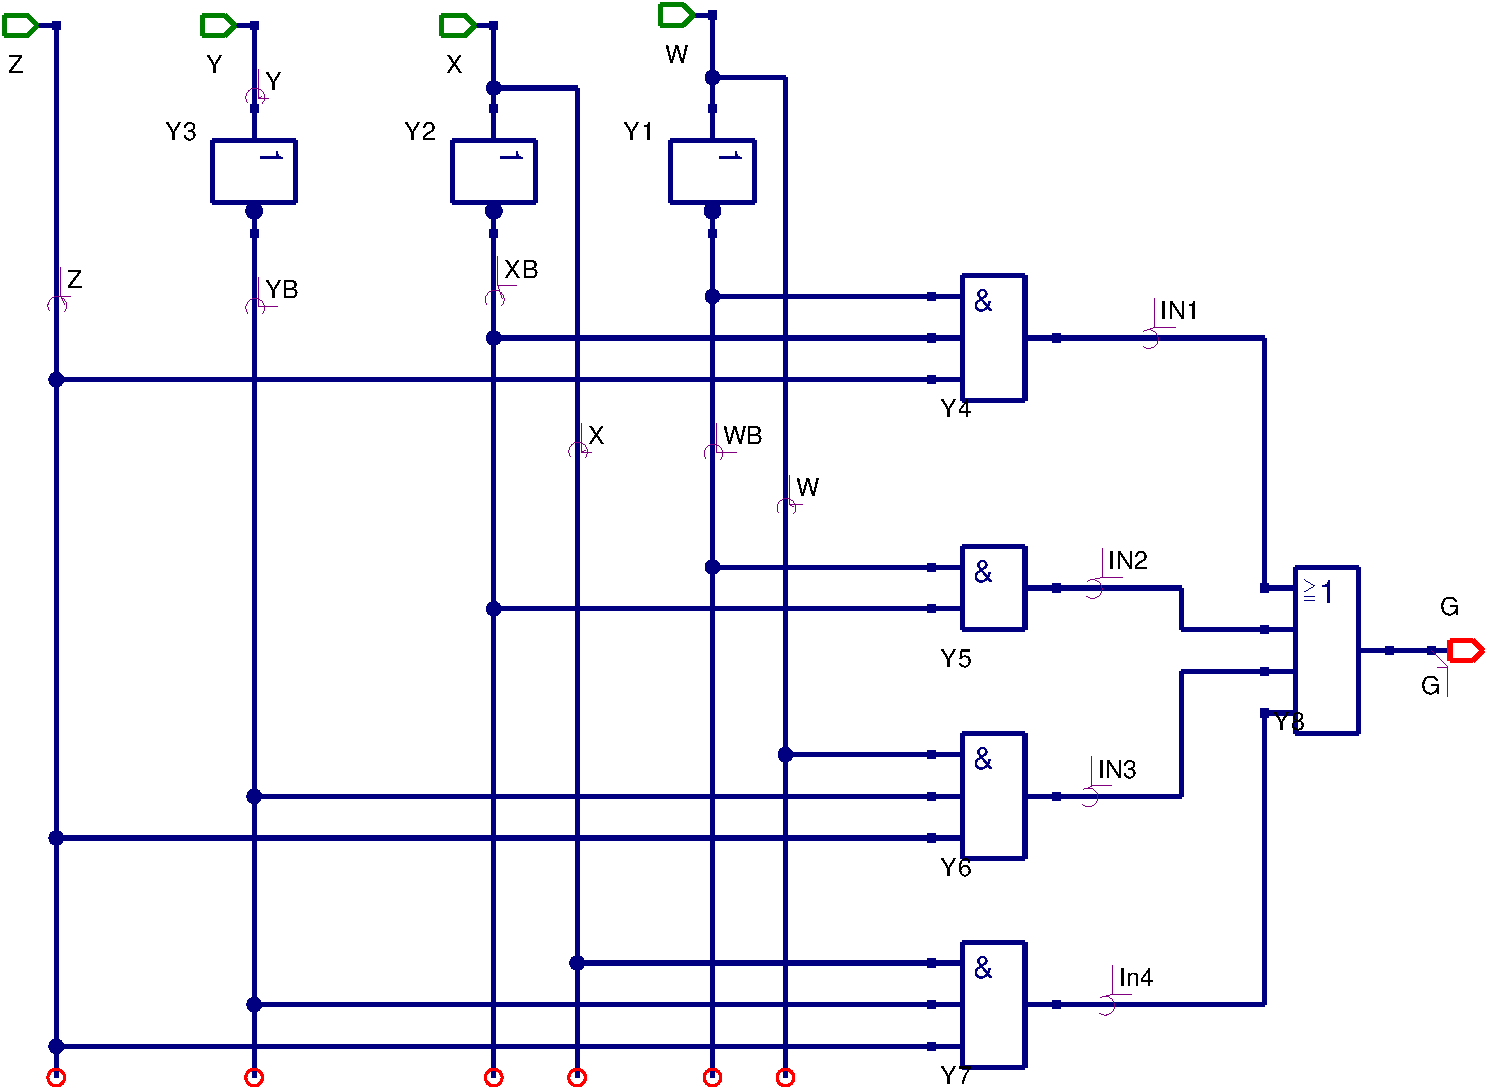
\includegraphics[width=0.8\linewidth]{t1ex2sch}
% tcomb1.png: 99.9998dpi, width=11.35cm, height=3.35cm, bb=0 0 447 132
  \caption{Combinational logic circuit with inputs W, X, Y, Z, and output G.}
  \label{fig:t1ex2sch}
\end{figure}
%\FloatBarrier

\addvspace{12pt}

After drawing a subcircuit schematic, input and output\footnote{Qucs
0.0.8 has a bug which causes a VHDL compile error when subcircuit pins
are specified as type out. A work around for this bug is to specify
subcircuit output pins as type analog.  The Qucs routines that
generate the circuit VHDL code convert pin type analog into VHDL type
inout. FreeHDL is then able to compile the generated VHDL code without
error. This bug has been corrected in Qucs 0.0.9.} pins are attached
to signal ports.  Input port pins of type in are shown on circuit
diagrams as a green symbol, signals W, X, Y, and Z, in
Fig.~\ref{fig:t1ex2sch}.  Ouput port pins of type out are coloured
red, signal G in Fig.~\ref{fig:t1ex2sch}. Signal flow through a port
is indicated by the direction of the port symbol arrow
head. Input/output signals, and any other signals that need to be
easily identified, are also named.  Once the subcircuit schematic is
complete, pressing key F3 causes Qucs to generate a subcircuit symbol.
The drawing tools listed as icons in the Qucs paintings window can be
used to edit Qucs generated subcircuit symbols.  The input/output port
pins on a subcircuit symbol have the same type and name as those on
the original subcircuit schematic.  Fig.~\ref{fig:comb1s} shows the
finished symbol for subcircuit COMB1. In these notes, symbol outlines
are shown drawn in accordance with the international code for logic
symbols\footnote{Ian, Kampel, A practical introduction to the new
logic symbols, Butterworths, 1985, ISBN 0-408-01461-X.}. To test our
new subcircuit we place it's symbol on a blank drawing sheet and apply
test signals to the input pins and observe the signals at the output
pin.  Fig.~\ref{fig:tcomb1s} shows a typical test circuit.  Subcircuit
Gen4bit generates a 4 bit test pattern synchronised to the input of a
digital clock. The specification for Gen4bit is given in the next
section of these notes\footnote{Subcircuit Gen4bit includes other
nested subcircuits.  Qucs 0.0.8 has a bug that causes VHDL compile
errors with some configurations of nested subcircuits. This has been
fixed in version 0.0.9. }.  The test pattern waveform and output
signal G are shown plotted as a function of time in
Fig.~\ref{fig:tcomb1}.

\begin{figure}
  \centering
  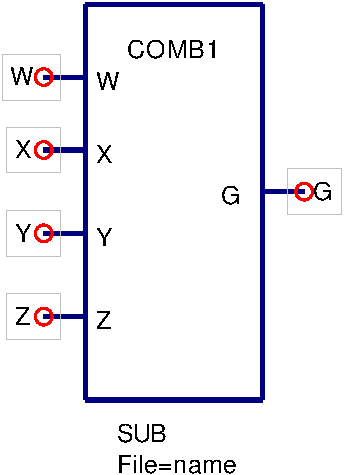
\includegraphics[width=0.2\linewidth]{comb1s}
% comb1s.png: 399.999dpi, width=2.72cm, height=3.92cm, bb=0 0 428 617
  \caption{Qucs symbol for a logic circuit with inputs W, X, Y, Z, and output G.}
  \label{fig:comb1s}
\end{figure}
\FloatBarrier

\begin{figure}
  \centering
  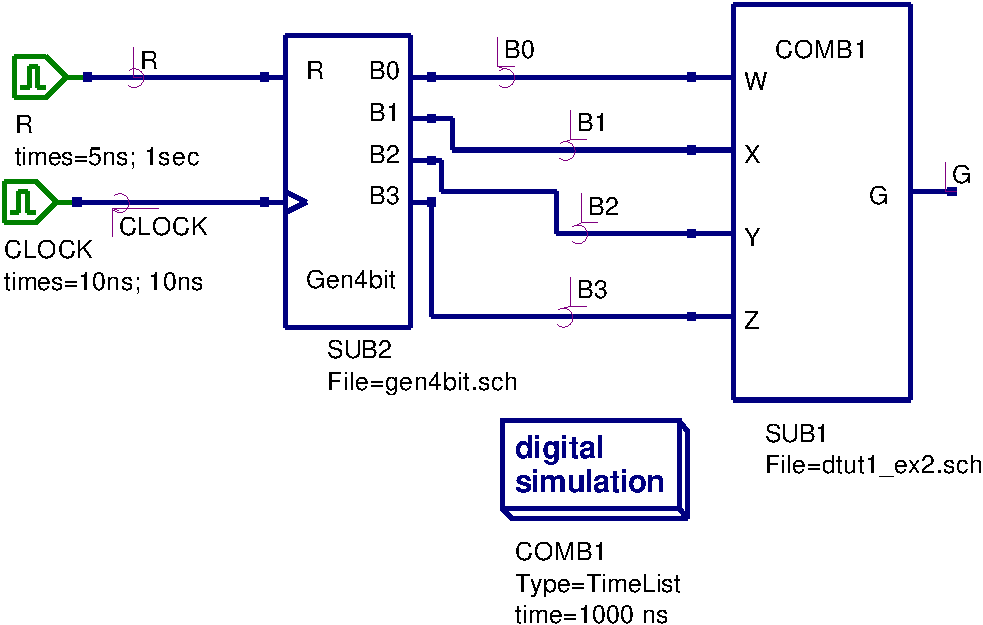
\includegraphics[width=0.8\linewidth]{tcomb1s}
% tcomb1s.png: 399.999dpi, width=7.44cm, height=4.72cm, bb=0 0 1172 743
  \caption{Test schematic for a logic circuit with inputs W, X, Y, Z, and output G.}
  \label{fig:tcomb1s}
\end{figure}
\FloatBarrier

\begin{figure}
  \centering
  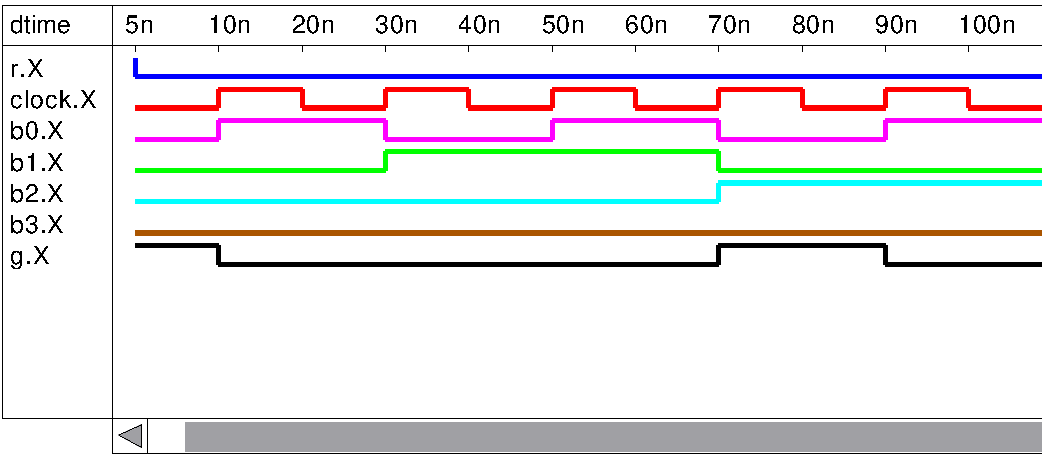
\includegraphics[width=0.9\linewidth]{tcomb1}
% tcomb1w.png: 399.999dpi, width=7.94cm, height=3.24cm, bb=0 0 1250 510
  \caption{Digital functional waveforms for a logic circuit with inputs W, X, Y, Z, and output G.}
  \label{fig:tcomb1}
\end{figure}
\FloatBarrier

\tutsection{Building a digital component library}

The Qucs graphical user interface includes good project handling
features.  Combining these features with the Qucs subcircuit
capabilities provides all the tools required for the development of a
library of common digital components.  Such a library can be stored in
a master project and the individual component files imported into
other projects when required.  Here are a few components that I
developed during a recent series of tests aimed at detecting bugs in
the VHDL code generated by Qucs.

\tutsubsection{Logic zero}

\begin{flushleft}
  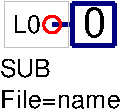
\includegraphics[width=.13\linewidth]{lzero} \hspace{10mm} 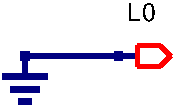
\includegraphics[width=0.23\linewidth]{lzerosch}
% lzerosch.png: 99.9998dpi, width=3.15cm, height=1.27cm, bb=0 0 124 50

% lzero.png: 99.9998dpi, width=1.50cm, height=1.45cm, bb=0 0 59 57
\end{flushleft}

\tutsubsection{Logic one}

\begin{flushleft}
  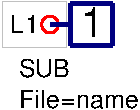
\includegraphics[width=.13\linewidth]{lone} \hspace{10mm} 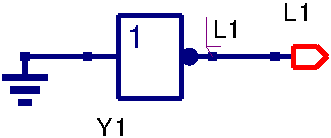
\includegraphics[width=0.23\linewidth]{lonesch}
% lonesch.png: 99.9998dpi, width=3.33cm, height=1.42cm, bb=0 0 131 56
\end{flushleft}

\tutsubsection{G2bit - 2 bit pattern generator}

\begin{center}
  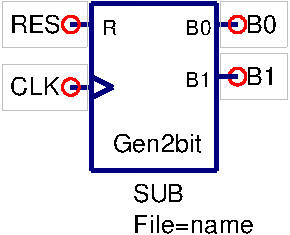
\includegraphics[]{g2bit} 
\end{center}
 \vspace{20mm}
\begin{center}
  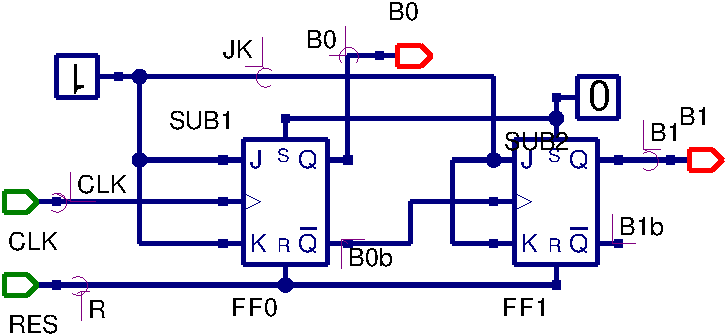
\includegraphics[width=0.8\linewidth]{g2bitsch}
\end{center}

\tutsubsection{G4bit - 4 bit pattern generator}

\begin{center}
  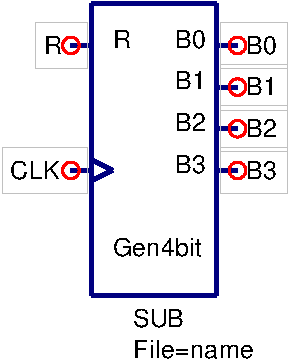
\includegraphics[]{g4bit}
\end{center}

\begin{center}
  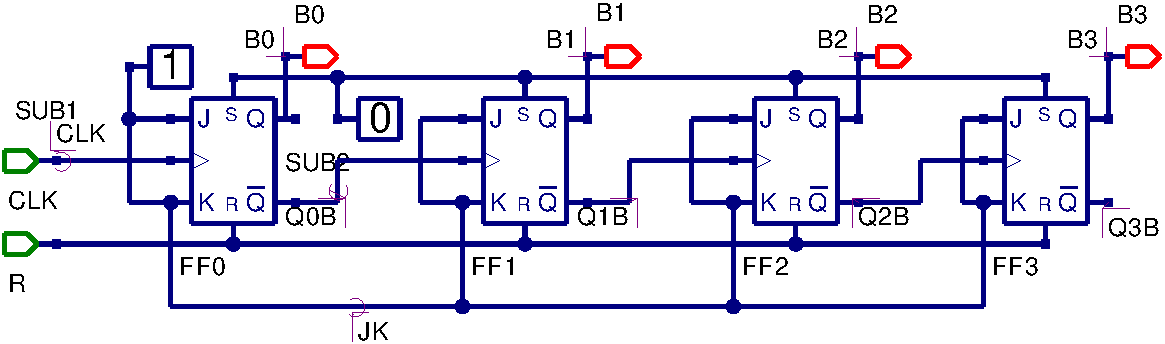
\includegraphics[width=1\linewidth]{g4bitsch}
% g4bit.png: 99.9998dpi, width=8.26cm, height=11.68cm, bb=0 0 325 460
\end{center}

\tutsubsection{MUX2to1 - 2 input to 1 output multiplexer}

\begin{center}
\begin{tabular}{lll}
EN & A & Y \\  
1 & X & L \\ 
0 & 0 & D0 \\ 
0 & 1 & D1
\end{tabular} 
\end{center}

\begin{center}
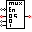
\includegraphics[]{mux2to1}
% mux2to1.png: 99.9998dpi, width=2.69cm, height=3.33cm, bb=0 0 106 131
\end{center}
\vspace{10mm}
\begin{center}
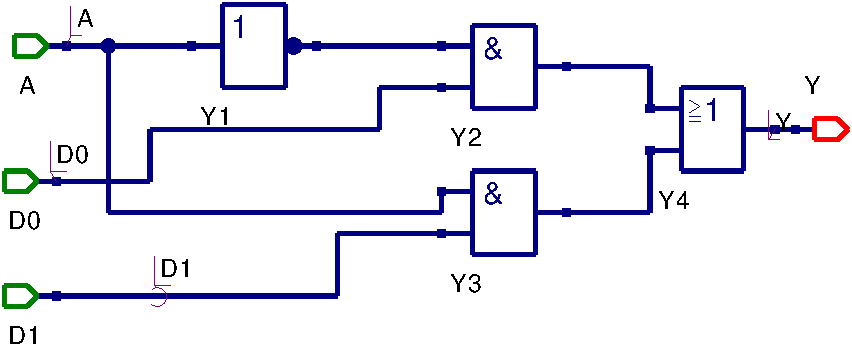
\includegraphics[]{mux2to1sch}
% mux2to1sch.png: 99.9998dpi, width=7.87cm, height=4.09cm, bb=0 0 310 161
\end{center}

\tutsubsection{MUX4to1 - 4 input to 1 multiplexer}

\vspace{5mm}
\begin{center}
\begin{tabular}{llll}
B & A & EN & Y \\ 
X & X & 1 & 0 \\ 
0 & 0 & 0 & D0 \\ 
0 & 1 & 0 & D1 \\ 
1 & 0 & 0 & D2 \\ 
1 & 1 & 0 & D3
\end{tabular}
\end{center}
\vspace{2mm}
\begin{center}
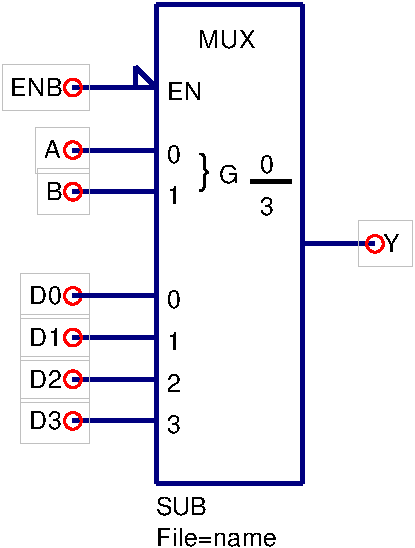
\includegraphics[width=0.3\linewidth]{mux4to1}
% mux4to1.png: 99.9998dpi, width=2.79cm, height=4.19cm, bb=0 0 110 165
\end{center}
\begin{center}
  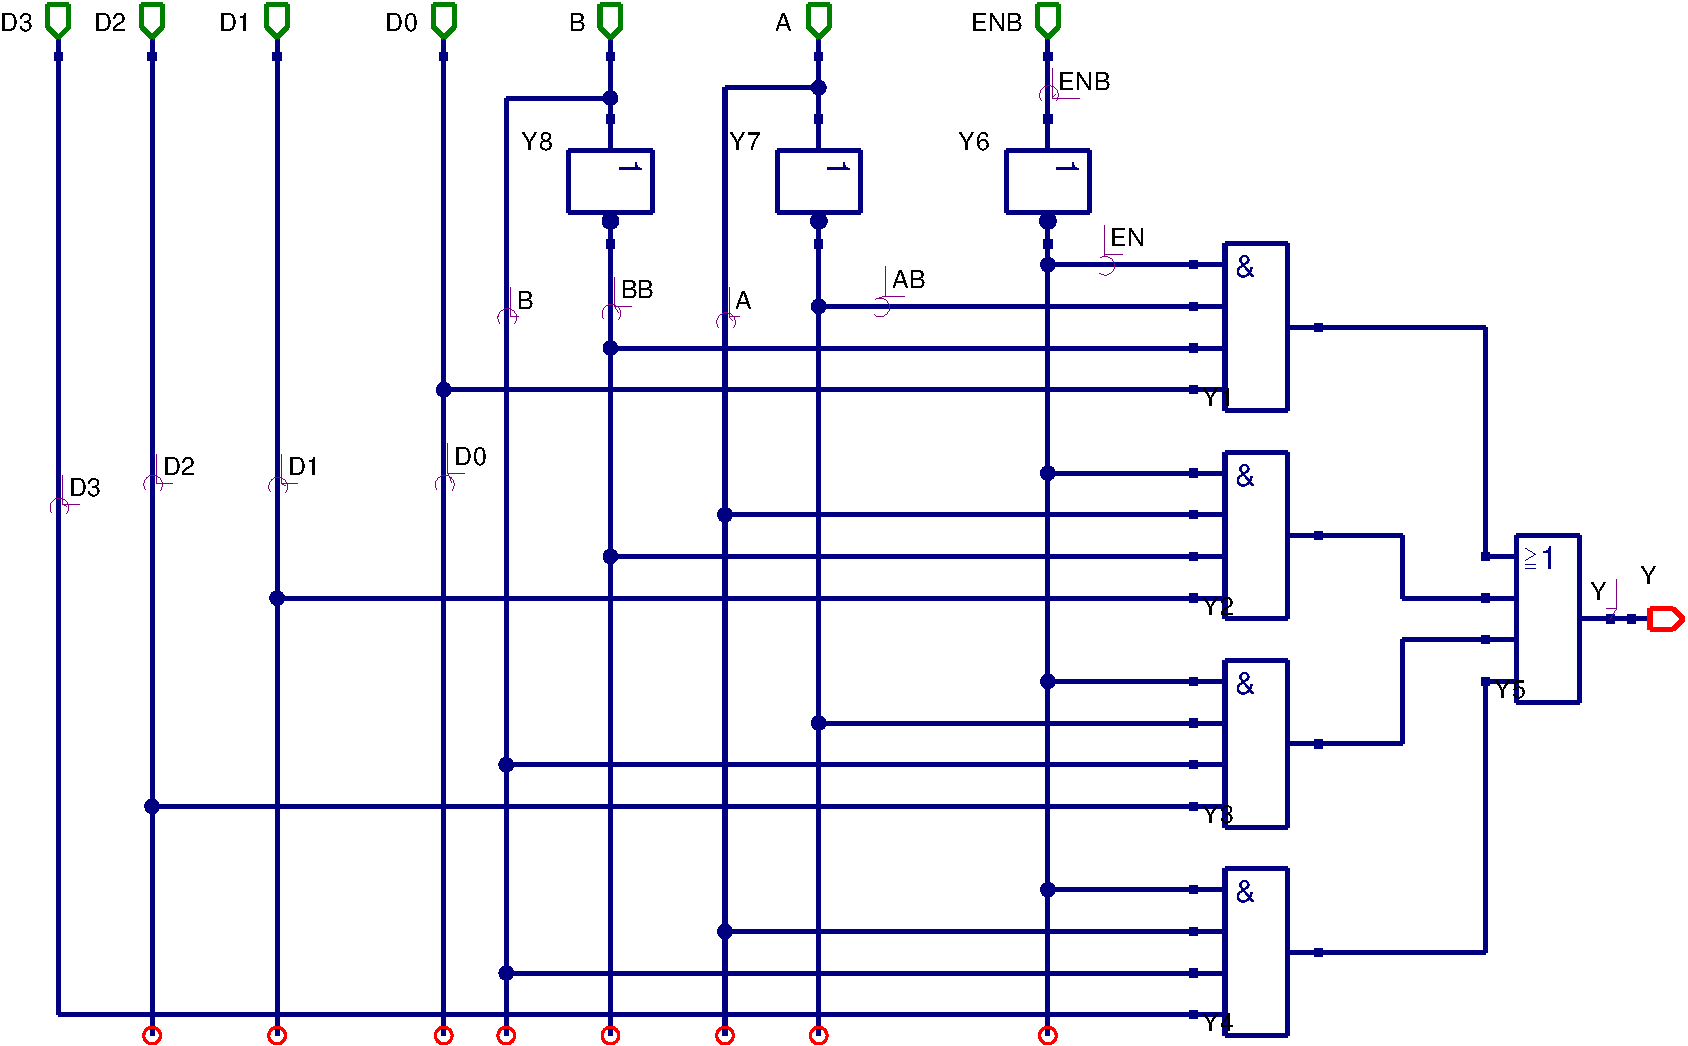
\includegraphics[width=1\linewidth]{mux4to1sch}
% mux4to1sch.png: 99.9998dpi, width=11.40cm, height=7.44cm, bb=0 0 449 293
\end{center}

\tutsubsection{2 bit adder}

\begin{center}
  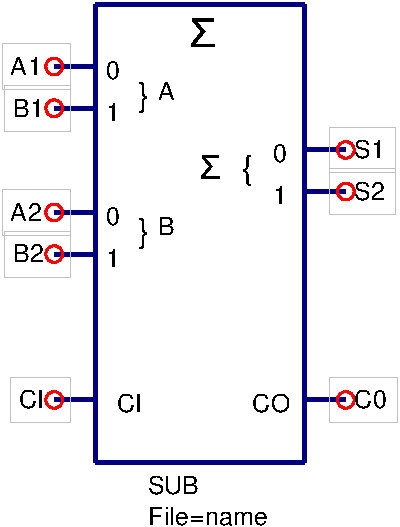
\includegraphics[width=0.3\linewidth]{fadder2bit}
% fadder2bit.png: 99.9998dpi, width=3.28cm, height=4.19cm, bb=0 0 129 165
\end{center}
\begin{center}
  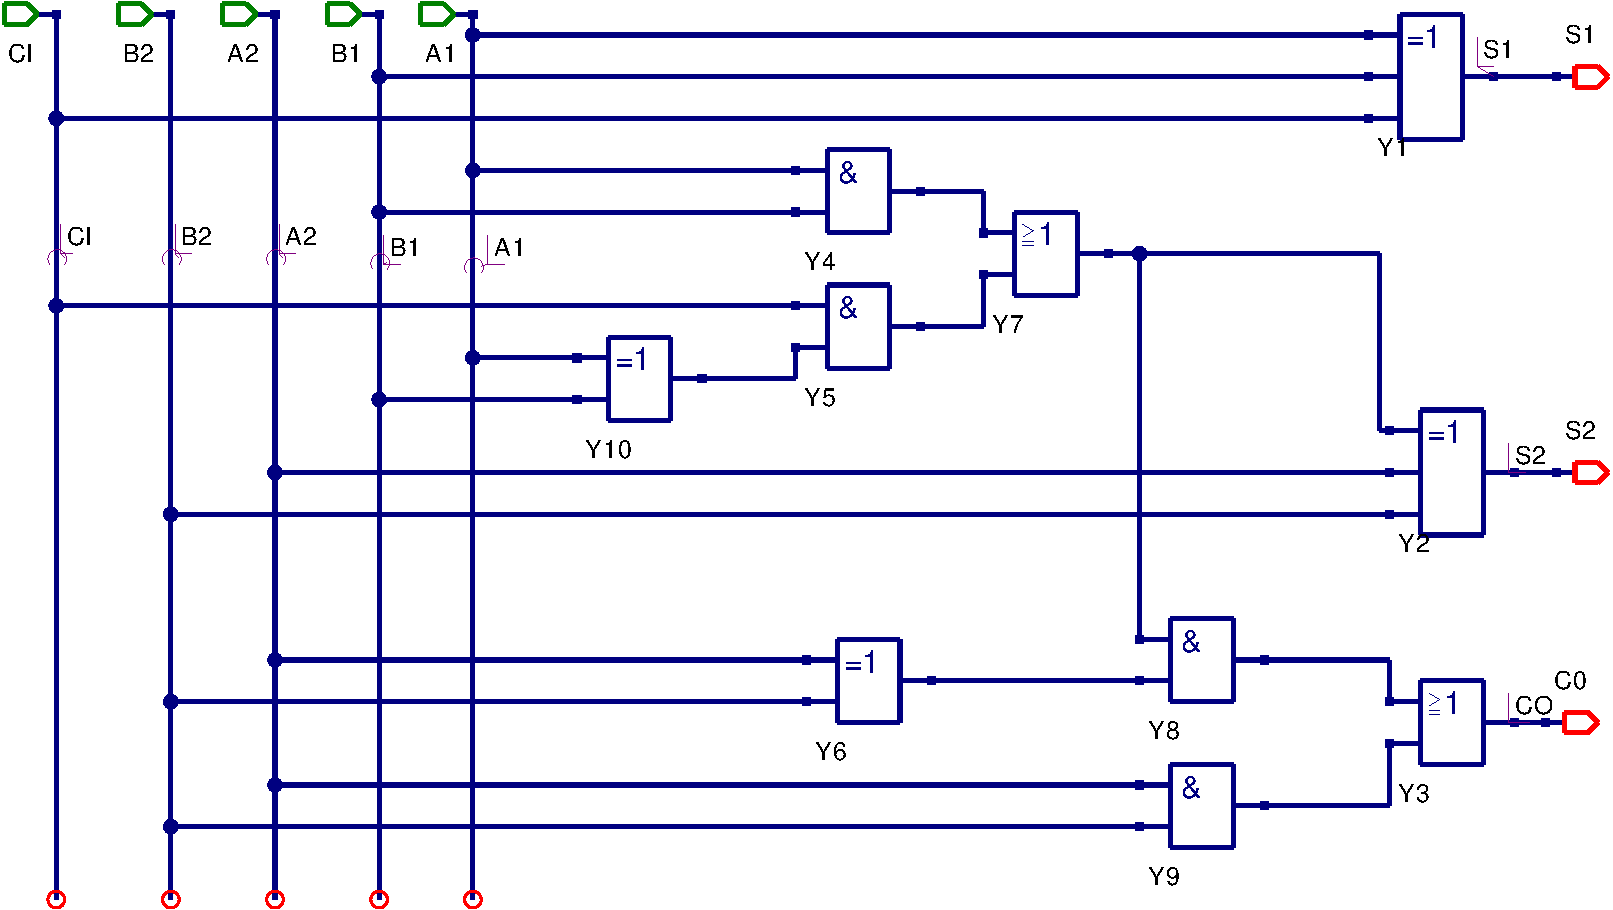
\includegraphics[width=1\linewidth]{fadder2bitsch}
% fadder2bitsch.png: 99.9998dpi, width=11.23cm, height=6.88cm, bb=0 0 442 271
\end{center}

\tutsection{Subcircuit VHDL code generated by Qucs}

Qucs generates a separate entity-architecture model for each
subcircuit.  These component definitions are compiled into the work
library by FreeHDL.  Here is the VHDL code from two of the previous
examples.

\tutsubsection{Gen2bit}

\begin{lstlisting}[
    language=VHDL,
    basicstyle=\small]
entity Sub_gen2bit is
  port (CLK: in bit;
        R: in bit;
        nnout_B0: out bit;
        nnout_B1: out bit);
end entity;
use work.all;
architecture Arch_Sub_gen2bit of Sub_gen2bit is
  signal B0b,
         B1b,
         JK,
         nnnet0,
         B0,
         B1 : bit;
begin
  FF0 : process (nnnet0, R, CLK)
  begin
    if (R='1') then  B0 <= '0';
    elsif (nnnet0='1') then  B0 <= '1';
    elsif (CLK='1' and CLK'event) then
      B0 <= (JK and not B0) or (not JK and B0);
    end if;
  end process;
  B0b <= not B0;

  FF1 : process (nnnet0, R, B0b)
  begin
    if (R='1') then  B1 <= '0';
    elsif (nnnet0='1') then  B1 <= '1';
    elsif (B0b='1' and B0b'event) then
      B1 <= (JK and not B1) or (not JK and B1);
    end if;
  end process;
  B1b <= not B1;

  SUB2: entity Sub_logic_zero port map (nnnet0);
  nnout_B0 <= B0 or '0';
  nnout_B1 <= B1 or '0';
  SUB1: entity Sub_Logic_one port map (JK);
end architecture;
\end{lstlisting}

\tutsubsection{2 bit adder}

\begin{lstlisting}[
    language=VHDL,
    basicstyle=\small]
entity Sub_fadd_2bit is
  port (A1: in bit;
        B1: in bit;
        A2: in bit;
        B2: in bit;
        CI: in bit;
        nnout_S1: out bit;
        nnout_S2: out bit;
        nnout_CO: out bit);
end entity;
use work.all;
architecture Arch_Sub_fadd_2bit of Sub_fadd_2bit is
  signal nnnet0,
         nnnet1,
         nnnet2,
         nnnet3,
         nnnet4,
         nnnet5,
         nnnet6,
         S2,
         CO,
         S1 : bit;
begin
  S1 <= CI xor B1 xor A1;
  nnnet0 <= B2 xor A2;
  nnnet1 <= nnnet0 and nnnet2;
  nnnet3 <= B2 and A2;
  nnnet2 <= nnnet4 or nnnet5;
  nnnet4 <= nnnet6 and CI;
  nnnet5 <= B1 and A1;
  S2 <= B2 xor A2 xor nnnet2;
  CO <= nnnet3 or nnnet1;
  nnnet6 <= B1 xor A1;
  nnout_S2 <= S2 or '0';
  nnout_CO <= CO or '0';
  nnout_S1 <= S1 or '0';
end architecture;
\end{lstlisting}

\tutsubsection{Notes on subcircuit VHDL generation}

\begin{itemize}
\item
Qucs predefined digital components generate concurrent data flow
signal statements or process statements.
\item
Previously defined subcircuit symbols generate VHDL port map
statements.
\item
 Type out entity port signals are prevented from being read as input
 signals by masking each output signal using the logic
 function  \textbf{signal-name OR '0'}.\footnote{Attempting to read
 entity port signals of type out results in a VHDL compile error. }
\item
 A VHDL \begin{lstlisting}[language=VHDL]
use work.all; \end{lstlisting}
statement is included before each subcircuit architecture definition
to ensure that FreeHDL can find any nested subcircuits
\footnote{Strictly speaking it should not be necessary to specifically
state the use of the work library as this library is normally visible
at all times when compiling entity-architecture models.  However, at
this stage in the development of FreeHDL it does appear that it is
necessary when using the default FreeHDL VHDL library mapping.}.
\item
The complete VHDL code file for a digital design is composed from an
outer test bench entity-architecture model plus entity-architecture
models for each subcircuit specified in the design,
\end{itemize}

\tutsection{Subcircuit nesting: A more complex design example}

In theory there is no limit to the depth of subcircuit nesting allowed
by Qucs.  In practice most digital circuit schematics can be
constructed with a maximum of four or five levels of design hierarchy.
Figure~\ref{fig:regt} shows an example that was used to test Qucs
subcircuit nesting performance.  The design is a simple RTL function
that uses a multiplexer to transfer data from one of two input
registers to a single output register.  The next section of these
notes outlines in detail the specification of the subcircuits needed
to build the RTL design.  A set of sample simulation waveforms showing the 
register transfer operation are illustrated in Fig.~\ref{fig:testrtl}.
\newpage 
\tutsubsection{4 bit RTL design}

\begin{figure}[ht]
  \centering
  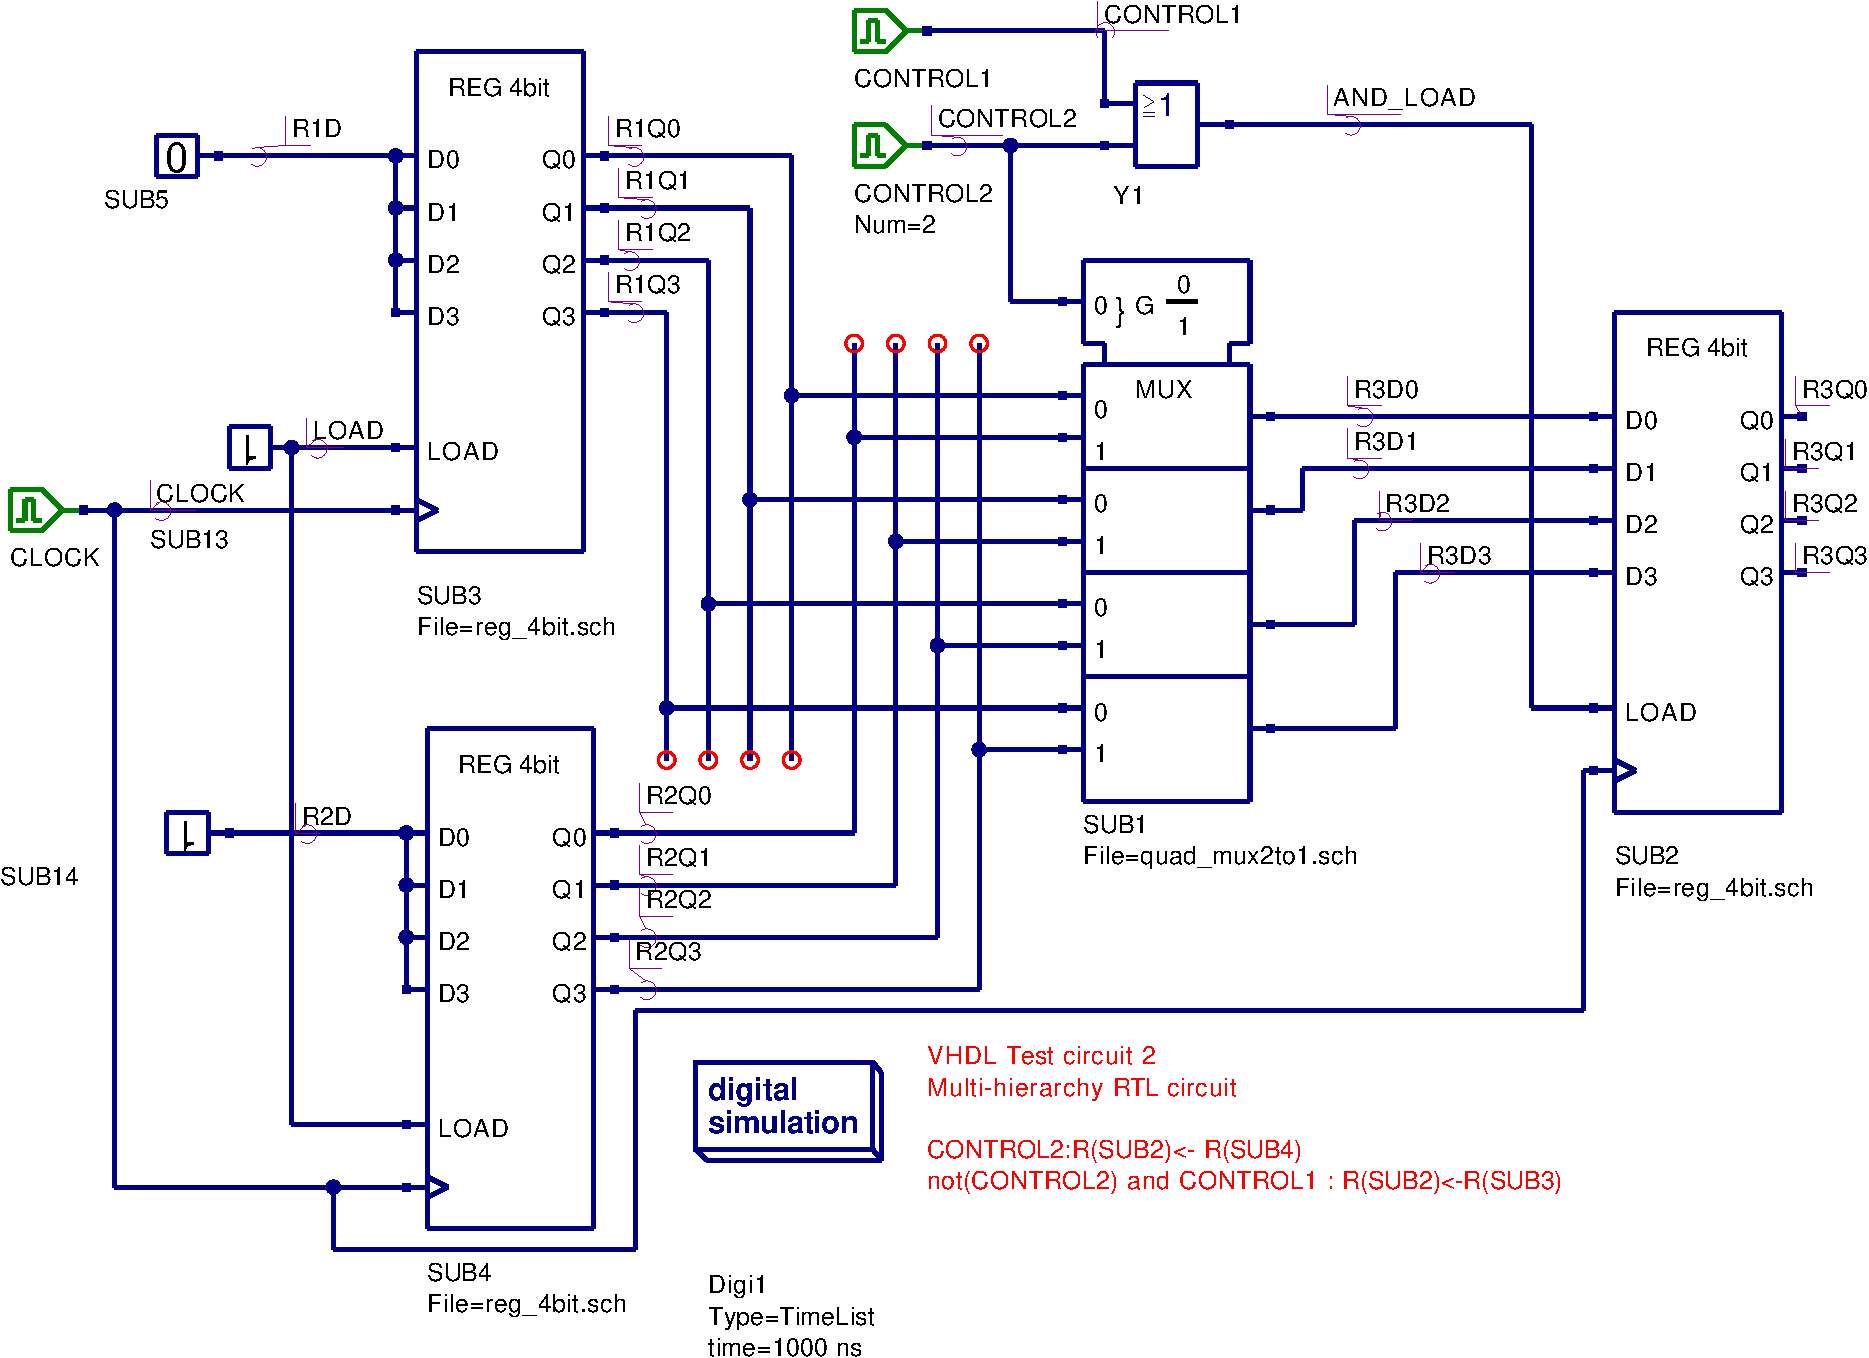
\includegraphics[width=1\linewidth]{regt}
% regt.png: 99.9998dpi, width=14.05cm, height=9.98cm, bb=0 0 553 393
  \caption{Top level schematic.}
  \label{fig:regt}
\end{figure} 
\FloatBarrier

\tutsubsubsection{Reg4bit}

	\begin{center}
	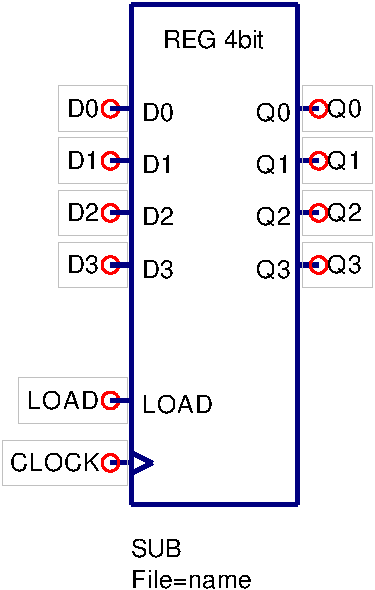
\includegraphics[width=.25\linewidth]{reg4bit}
% reg4bit.png: 99.9998dpi, width=2.69cm, height=4.32cm, bb=0 0 106 170
	\end{center}
\vspace{10mm}
	\begin{center}
	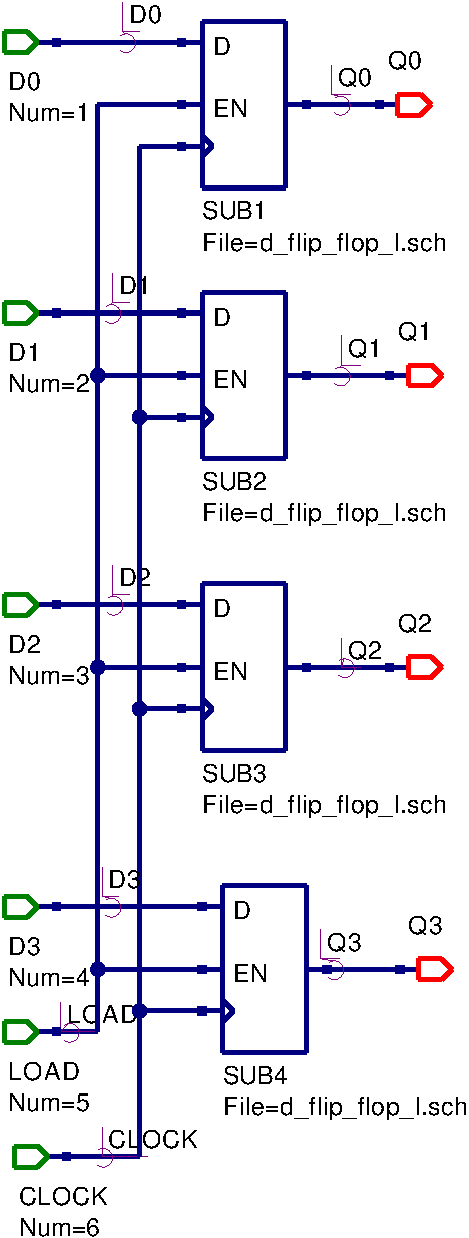
\includegraphics[width=.3\linewidth]{reg4bitsch}
% reg4bitsch.png: 99.9998dpi, width=6.38cm, height=13.72cm, bb=0 0 251 540
	\end{center}
\pagebreak
\tutsubsubsection{D flip-flop with load enable}
	\begin{center}
	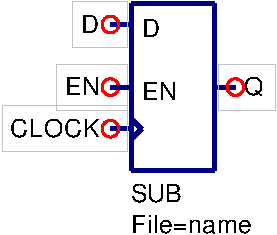
\includegraphics[width=0.2\linewidth]{dffl}
% dffl.png: 99.9998dpi, width=2.31cm, height=2.44cm, bb=0 0 91 96
	\end{center}

	\begin{center}
	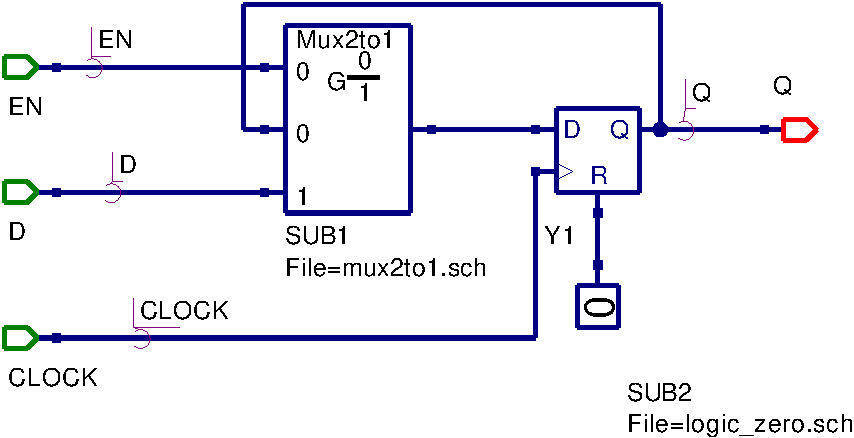
\includegraphics[width=0.7\linewidth]{dfflsch}
% dfflsch.png: 99.9998dpi, width=5.99cm, height=3.30cm, bb=0 0 236 130
	\end{center}
\tutsubsubsection{Mux2to1}
	\begin{center}
	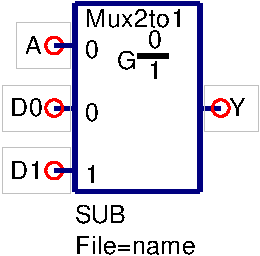
\includegraphics[width=0.2\linewidth]{mux21}
% mux21.png: 99.9998dpi, width=2.34cm, height=2.31cm, bb=0 0 92 91
	\end{center}
	\begin{center}
	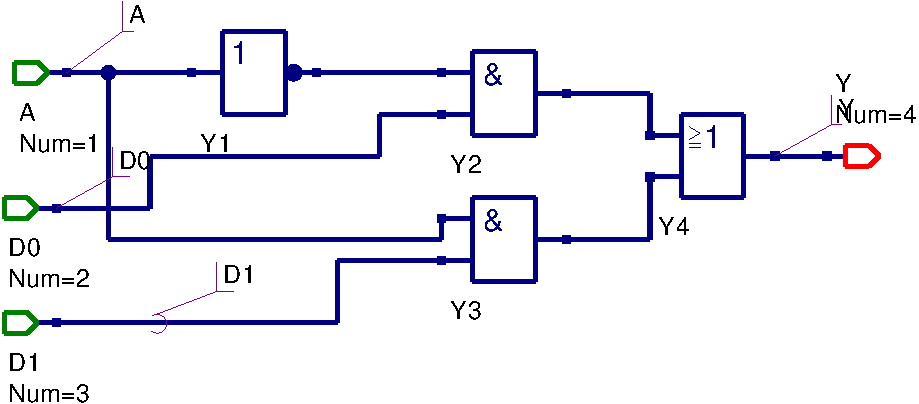
\includegraphics[width=0.7\linewidth]{mux21sch}
% mux21sch.png: 99.9998dpi, width=6.43cm, height=2.97cm, bb=0 0 253 117
	\end{center}
\tutsubsubsection{QuadMux}
	\begin{center}
	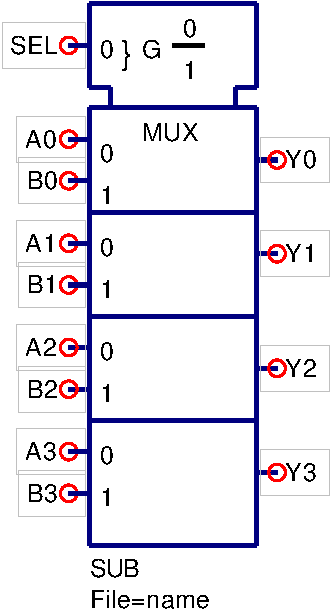
\includegraphics[width=0.2\linewidth]{quadmux}
% quadmux.png: 99.9998dpi, width=2.92cm, height=4.50cm, bb=0 0 115 177
	\end{center}
	\begin{center}
	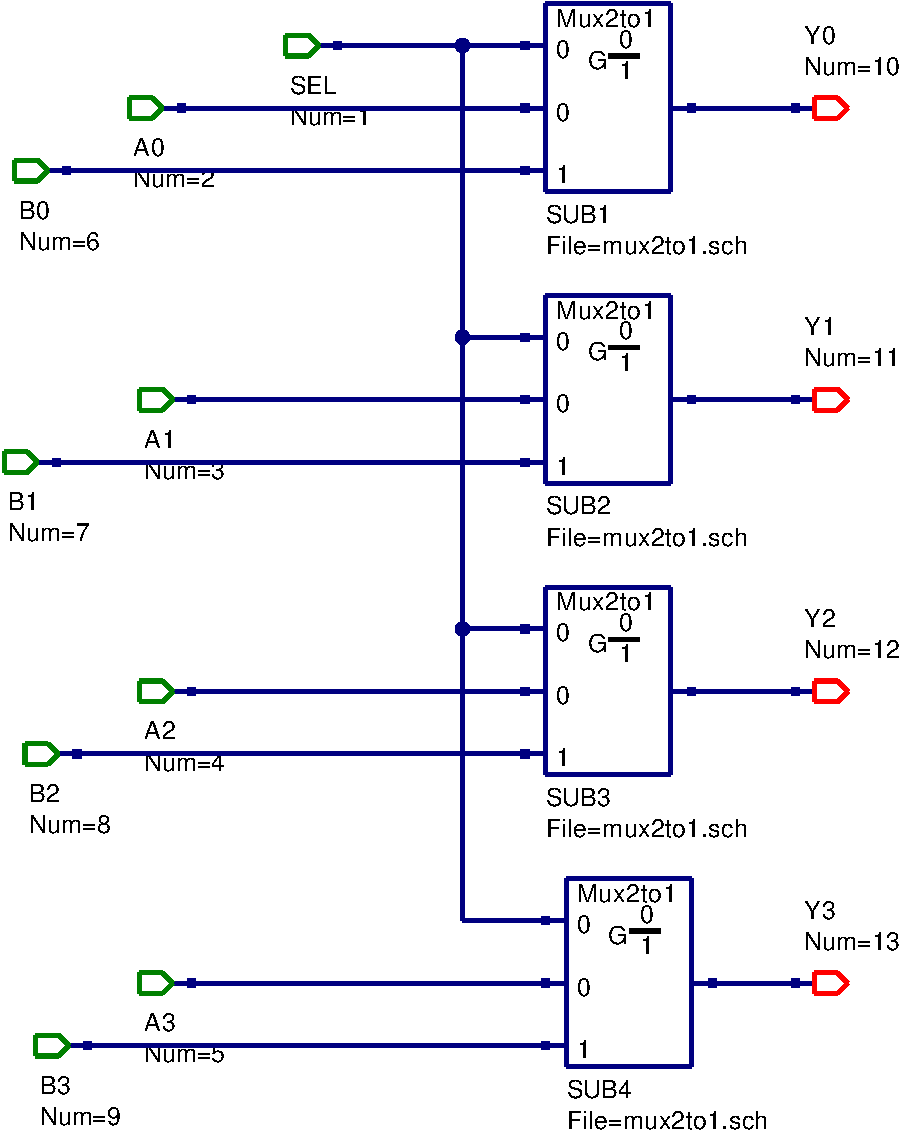
\includegraphics[width=0.7\linewidth]{quadmuxsch}
% quadmuxsch.png: 99.9998dpi, width=6.43cm, height=7.85cm, bb=0 0 253 309
	\end{center}

\begin{figure}[ht]
  \centering
  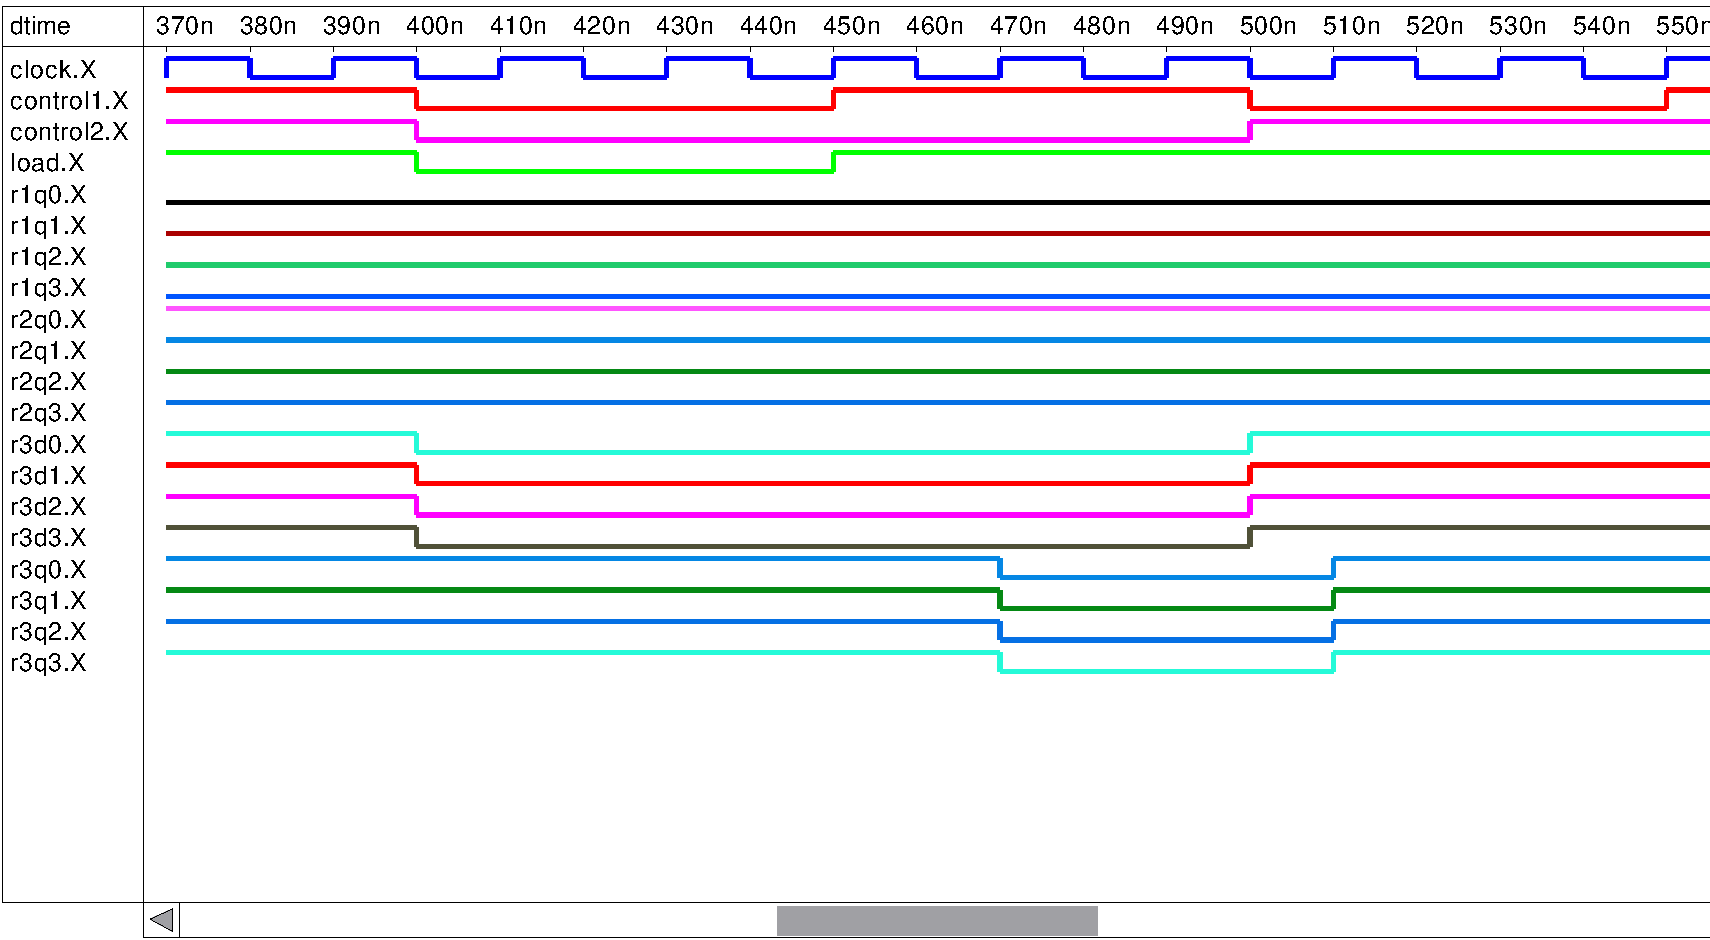
\includegraphics[width=0.9\linewidth]{testrtl}
% quadmuxdpl.png: 99.9998dpi, width=11.40cm, height=6.63cm, bb=0 0 449 261
  \caption{Sample simulation waveforms for RTL design.}
  \label{fig:testrtl}
\end{figure} 
\FloatBarrier

\tutsection{Update number one: May 2006}

Although it is only a short time since the first version of these
digital tutorial notes was posted on the Qucs Sourceforge Web site,
much has happened in the world of Qucs digital simulation.  Bugs in
the Qucs code have been found, and fixed, and a range of new features
added to the software. These expand the power of Qucs digital
simulation and give users a glimpse of how the package will evolve in
the future.  The purpose of these notes is firstly to update readers
as to the changes to Qucs digital simulation and secondly to explain
how to use the new Qucs features.  Please note however, they are not
intended to teach readers how to program using VHDL.\footnote{A good
introduction to the VHDL language and it's application in digital
system design can be found in \textbf{\textit{Digital System Design
using VHDL}} by Charles H. Roth, Jr, PWS Publishing Company, 1997,
ISBN 0-534-95099-X. }

\tutsubsection{Bugs, corrections and small changes to the Qucs digital simulation code}

All the bugs reported in the first version of these notes have been
corrected in the latest Qucs CVS code.  These corrections are, of
course, also included in Qucs release 0.0.9. During testing a number
of other annoying, but significant, bugs have also been found and
eliminated, these include

\begin{itemize}
\item
Multiple input gates (three or more inputs) of types nand and nor
failed at the FreeHDL compile stage due to an error in the VHDL code
generated by Qucs.
\item
Signals names and, for example, component names constructed from a
single letter that was an abbreviation for a physical unit failed to
compile.
\item
Changing digital component time delays caused component connections on
a sche\-ma\-tic to be removed.
\item
GUI problems caused by errors in the symbol rotation and mirror code.
\item
Qucsconv code conversion errors caused the Qucs digital simulation
cycle to fail before plotting TimeList waveforms.
\end{itemize}

A number of changes to either the VHDL code generated by Qucs or the
schematic capture GUI have been introduced, these include

\begin{itemize}
\item The VHDL code generated by Qucs for the ground symbol has been changed from
\begin{lstlisting}[language=VHDL]
gnd <= gnd and '0';
\end{lstlisting}
to
\begin{lstlisting}[language=VHDL]
gnd <= '0';
\end{lstlisting}
\item The symbol for digital inout ports has been changed from the analogue pin symbol to one that consists of the digital in and out pins drawn back-to-back.  This reflects the bidirectional status of an inout port.
\end{itemize}

A more complete list of all the bug corrections and other program
modifications can be found in the Qucs change log files.

\tutsubsection{New digital simulation features}

The flow diagram illustrated in Fig.~\ref{fig:digital_ud1_fa} shows a
number of different simulation routes for a digital circuit under
test.  The Qucs digital simulation facilities have been improved to
include direct simulation of VHDL testbench code and the simulation of
circuit schematics that include digital components specified by VHDL
entity-architecture models.  The various combinations that users can
adopt for Qucs digital circuit entry are as follows:

\begin{enumerate}
\item Schematic circuit entry using predefined digital component symbols, subcircuits generated using the same symbols and a copy of the digital simulation icon; this is the approach described in the first version of these tutorial notes.
\item Circuit entry identical to 1 plus symbols for digital components specified by VHDL entity-architecture models.
\item Circuit entry using the Qucs VHDL code editor. The text entered describes both the circuit under test and the test vectors needed to drive the circuit inputs during simulation. 
\end{enumerate}
Once the circuit under test has been entered into Qucs, clicking the
Simulate menu button, or pressing key F2, starts the Qucs digital
simulation process.

\begin{figure}
  \centering
  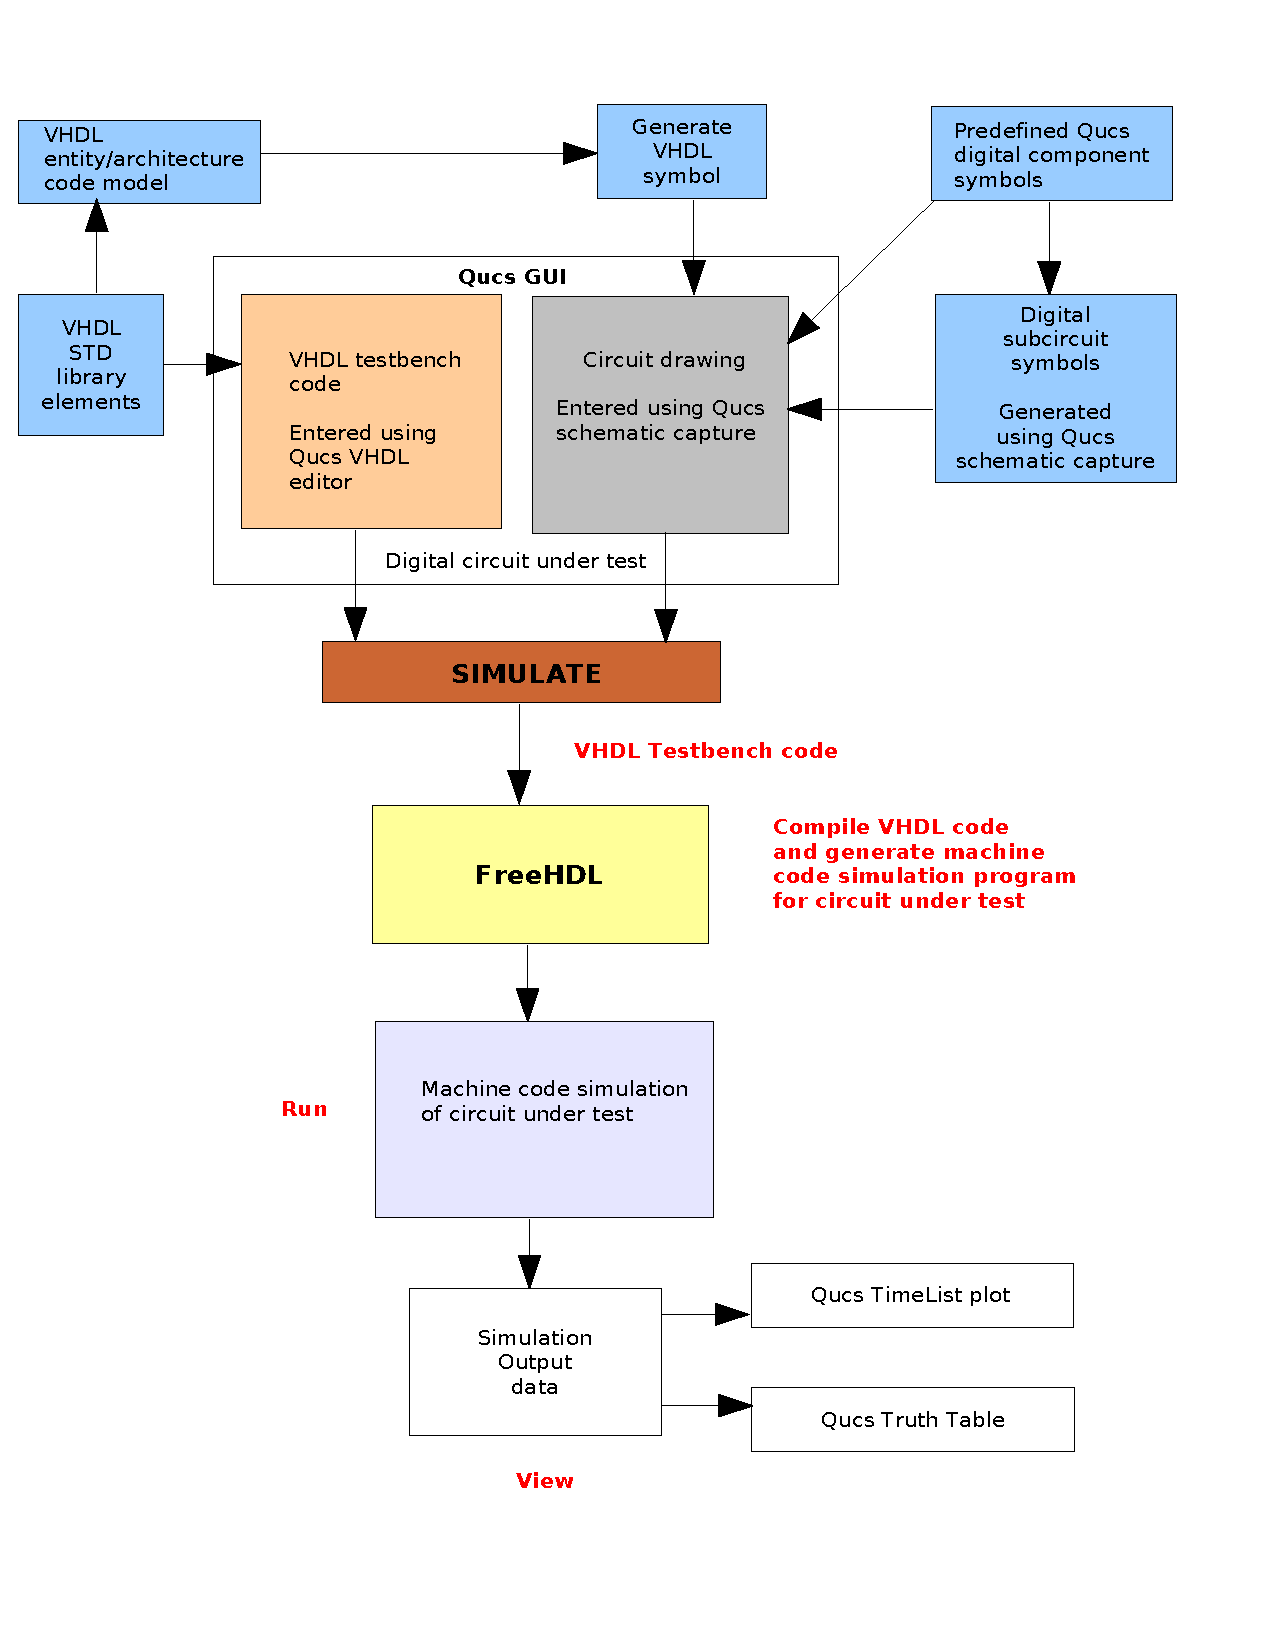
\includegraphics[width=0.99\linewidth]{digital_ud1_fa}
  \caption{Flow diagram of Qucs digital simulation routes.}
  \label{fig:digital_ud1_fa}
\end{figure} 

\tutsubsection{Limitations}

Before describing the new digital simulation features it is important
that readers understand the limitations that are inherent in the
various digital simulation routes described in the last section and
illustrated in the flow diagram shown in
Fig.~\ref{fig:digital_ud1_fa}.  Qucs schematic capture allows users to
draw circuits consisting of predefined component symbols and
subcircuit symbols.  At this stage in the development of the GUI
digital signals must be of type bit (as defined in the VHDL standard
library - library STD in the FreeHDL package) where individual signals
flow through a single wire.  Qucs schematic drawing bus structures of
VHDL type bit-vector, for example, have not been implemented yet.
This implies that the device symbol port pins must represent single
signals.  Similarly the nets connecting pins on more than one device
can only be single signal nets and not bus structures.  It is
anticipated that this will change in a future Qucs release.

\addvspace{12pt}

Although the current release of FreeHDL is 0.0.1 the package
implements a substantial subset of the entire VHDL language\footnote{A
complete description of the 1987 and 1993 specifications of the VHDL
language can be found in The Designer's Guide to VHDL by Peter J
Ashenden, second edition 2002, Morgan Kaufmann Publishers, ISBN
1-55860-674-2. }.  The major features not supported by release 0.0.1
are:
\begin{itemize}
\item Shared variables.
\item The following attributes; transaction, quiet, stable and delayed.
\item User defined attributes.
\item Groups.
\item Guarded signal assignments.
\item Currently drivers cannot be switched off.
\end{itemize}

The Qucs TimeList plotting program uses signal data output by the
machine code simulation program generated by the FreeHDL
package\footnote{The machine code simulation program outputs signal
data in VCD format.  This is then converted to the Qucs TimeList data
format by the qucsconv utility program.}.  A current limitation of the
TimeList plotting program is that it can only display signals of type
bit. Bus signal waveforms cannot be displayed.

\addvspace{12pt}

Given the above limitations it is therefore possible to write VHDL
code that can be compiled by FreeHDL but will cause problems at either
the schematic drawing or output waveform plotting stages in the Qucs
simulation cycle.  As Qucs develops it is expected that these
limitations will be removed.  On the subject of limitations one final
point to note: FreeHDL can simulate circuits described by the data
types and other features found in the
\begin{verbatim}
  IEEE.std_logic_1164
\end{verbatim} 
library and other predefined libraries.  However, at this stage in the
development of the Qucs software only the VHDL standard library may be
used, implying that data type bit must be used to represent logic
signals.

\tutsubsection{Using the Qucs VHDL editor}

Qucs release 0.0.9 includes a VHDL text editor\footnote{To launch the
new VHDL editor click on the second icon from the left on the Qucs
toolbar. It can also be activated using the key sequence
Ctrl+Shift+V.} that has all the usual edit features plus colour coding
of the various VHDL language statements.  One unusual feature of this
editor is a zoom control that allows the text size to be increased or
decreased in a similar way to the schematic drawing zoom.  The VHDL
editor is included in the Qucs package for two primary purposes,
firstly for purely text file VHDL simulation\footnote{This is still
the preferred method amongst many experienced users of VHDL.  However,
the circuit schematic drawing approach does seem to be growing in
popularity.  } and secondly for the development of VHDL
entity-architecture models that can be linked to schematic capture
symbols.  The latter increases significantly the capabilities of the
Qucs software in that it allows libraries of hand-crafted device
models to be constructed.  These new library devices will, given
support by the general Qucs user community, greatly expand the
potential use of the Qucs package.  In this section the use of the
VHDL text editor is demonstrated through a series of digital circuit
simulation examples. The included VHDL listings indicate typical Qucs
use of a number of the basic VHDL data types. The text also outlines
any limitations imposed by Qucs.
 
\begin{itemize}
\item Example 1: A sum of products (SOP) combinational digital circuit.

The Boolean equation\footnote{The Boolean equation for function f has
not been minimised.  It is in a form derived directly from a truth
table and is introduced purely as an example to demonstrate the use of
the Qucs VHDL editor.} for a SOP combinational circuit is:
\begin{center}
\begin{large}$f=\overline{W}.X.\overline{Y}.\overline{Z}+\overline{W}.\overline{X}.\overline{Y}.\overline{Z}+W.\overline{Y}.\overline{Z}+W.X.Y.Z$\end{large}
\end{center}

The VHDL code for a structural model of this combinational circuit and
its associated testbench is given in the following listing.

\begin{lstlisting}[
    language=VHDL,
    basicstyle=\small]
-- Qucs VHDL editor example 1
--
entity test_vector is  -- Test vector generator.
	port( z, y, x, w : out bit
	      );
end entity test_vector;
--
architecture behavioural of test_vector is
begin 
pz : process is
	begin 
		z <= '0' ; wait for 20 ns;
		z <= '1' ; wait for 20 ns;
      end process pz;
py : process is
	begin 
		y <= '0' ; wait for 40 ns;
		y <= '1' ; wait for 40 ns;
      end process py;
px : process is
	begin 
		x <= '0' ; wait for 80 ns;
		x <= '1' ; wait for 80 ns;
      end process px;
pw : process is
	begin 
		w <= '0' ; wait for 160 ns;
		w <= '1' ; wait for 160 ns;
      end process pw;
end architecture behavioural;
--
entity and4 is -- 4 input and gate.
	port( in1, in2, in3, in4 : in bit;
	        out1 : out bit
	       );
end entity and4;
--
architecture dataflow of and4 is
begin 
	out1 <= in1 and in2 and in3 and in4;
end architecture dataflow;
--
entity and3 is -- 3 input and gate.
	port( in1, in2, in3  : in bit;
	        out1 : out bit
	       );
end entity and3;
--
architecture dataflow of and3 is
begin 
	out1 <= in1 and in2 and in3;
end architecture dataflow;
--
entity or4 is -- 4 input or gate.
	port( in1, in2, in3, in4 : in bit;
	        out1 : out bit
	       );
end entity or4;
--
architecture dataflow of or4 is
begin 
	out1 <= in1 or in2 or in3 or in4;
end architecture dataflow;

entity inv is -- Inverter.
	port( in1 : in bit;
	        out1 : out bit
	       );
end entity inv;
--
architecture dataflow of inv is
begin 
	out1 <= not in1;
end architecture dataflow;
--
entity testbench is  --  Test bench outer entity wrapper.
end entity testbench;
--
library work;
use work.all;
--
architecture structural of testbench is  -- Testbench architecture.
signal b0, b1, b2, b3, zb, yb, xb, wb,a, b, c, d, f : bit;
begin
	d1 : entity test_vector port map(b0, b1, b2, b3);
	d2 : entity inv port map(b0, wb);
	d3 : entity inv port map(b1, xb);
	d4 : entity inv port map(b2, yb);
	d5 : entity inv port map(b3, zb);
	d6 : entity and4 port map(zb, yb, b1, wb, a);
	d7 : entity and4 port map(zb, yb, xb, wb, b);
	d8 : entity and3 port map(zb, yb, b0, c);
	d9 : entity and4 port map(b0, b1, b2, b3, d);
	d10 : entity or4 port map(a, b, c, d, f);
end architecture structural;
\end{lstlisting}

On entry of this code into the Qucs VHDL text editor the text is
colour coded.  Unfortunately, the colour coding is lost when printed,
or pasted into a word processor, or a layout package like LaTeX.  The
structure of the VHDL listing follows the normal convention for text
based VHDL simulation.  All component entity-architecture models must
be defined before they are referenced in other component models. The
simulation test bench must be the last entity-architecture model in
the VHDL listing.  During the VHDL compile phase FreeHDL compiles the
component entity-architecture models to the work library\footnote{In
most VHDL implementations library work is always visible and there is
no requirement to make it visible by using the library and use
statements.  However, FreeHDL appears to need these statements at the
linking phase otherwise the VHDL compiler fails.  }.  These compiled
models are then made available to the simulation test bench through
the use of the VHDL\textbf{\textit{ use}} statement inserted in the
listing prior to the testbench architecture statement.  Once the VHDL
listing for the simulation has been typed into the Qucs VHDL code
editor, pressing key F2 starts the simulation process.  The simulation
duration can be set using the Document Settings in the File dropdown
menu (or by pressing the Ctrl+. keys).  Any VHDL syntax errors, or
indeed typos, are written to file and can be viewed by pressing key
F5.  Obviously if errors are reported these need to be corrected using
the VHDL text editor and the simulation cycle restarted.  A typical
TimeList output for editor example 1 is shown in
Fig.~\ref{fig:dig_ud1_ex1_dpl}.

 \begin{figure}[ht]
  \centering
  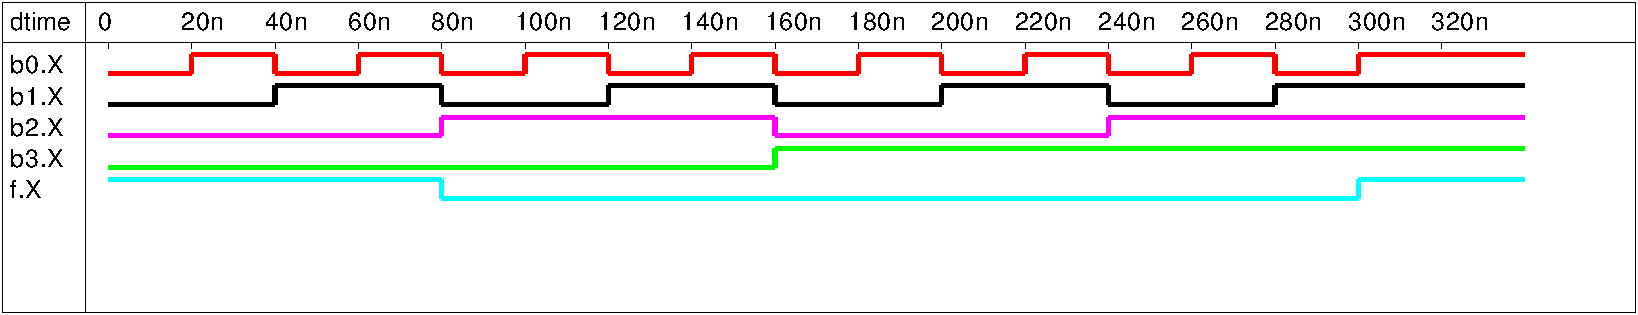
\includegraphics[width=1\linewidth]{dig_ud1_ex1_dpl}
  \caption{Sample simulation waveforms for VHDL editor example 1 design.}
  \label{fig:dig_ud1_ex1_dpl}
\end{figure} 

\end{itemize}

\begin{itemize}
\item Example 2: VHDL editor example 1 modelled using dataflow VHDL statements.

The VHDL code for the second example is given in the next listing.
The VHDL style chosen to model the circuit is based on VHDL dataflow
concurrent signal assignments.  The input text vectors are generated
using a simple state machine rather than separate process statements.
The test vector generator port specification uses entirely single
signal bit types and can be easily interfaced, without problems, to
other components connected on a Qucs schematic diagram.  The procedure
for generating schematic capture component symbols from entity -
architecture models is introduced in a later section of these notes.
The use of bit vector bus constructions is also illustrated in this
example.  Qucs allows the use of bit vectors as signals or variables
in VHDL models provided all signals in the port statement of entity
declaration are of type bit only.\footnote{This is a restriction of
Qucs 0.0.9 and will be removed in a later release of the package. Also
note signals of type bit vector that are declared in architecture
definitions are listed in the TimeList plot signal dialogue. However,
a text message saying no data results if an attempt is made to display
them.  Again this limitation will be removed in a later release of
Qucs.}  A typical TimeList output for editor example 2 is shown in
Fig.~\ref{fig:dig_ud1_ex2_dpl}.

\begin{lstlisting}[
    language=VHDL,
    basicstyle=\small]
-- Qucs VHDL editor example 2
--
entity test_vector_a is
	port( RESET, CLOCK : in bit;
	      B0, B1, B2, B3 : out  bit
	    );
end entity test_vector_a;
--
architecture behavioural of test_vector_a is
signal present_state, next_state : bit_vector(3 downto 0):="1111";
begin
--
p1 : process(CLOCK ) is
        begin
          if  (CLOCK'event and CLOCK='1') then
             present_state <= next_state;
          end if;
       end process p1;
--      
p2 : process(RESET,  present_state) is
        begin	
         if (RESET = '1' ) then next_state <= "1111"; 
         end if;
        case present_state is
	 when "0000" =>  next_state <= "0001";   
	 when "0001"  =>  next_state <= "0010"; 
	 when "0010"  =>  next_state <= "0011";  
	 when "0011"  =>  next_state <= "0100";   
	 when "0100"  =>  next_state <= "0101";   
	 when "0101"  =>  next_state <= "0110";   
	 when "0110"  =>  next_state <= "0111";   
	 when "0111"  =>  next_state <= "1000";   
	 when "1000"  =>  next_state <= "1001";   
	 when "1001"  =>  next_state <= "1010"; 
	 when "1010"  =>  next_state <= "1011"; 
	 when "1011"  =>  next_state <= "1100"; 
	 when "1100"  =>  next_state <= "1101"; 
	 when "1101"  =>  next_state <= "1110"; 
	 when "1110"  =>  next_state <= "1111"; 
	 when "1111"  =>  next_state <= "0000";
	end case;
          B3 <= next_state(3); B2 <= next_state(2); 
          B1 <= next_state(1); B0 <= next_state(0);
     end process p2;
end architecture behavioural;
--
library work;
use work.all;
--
entity testbench is
end entity testbench;
--
architecture dataflow of testbench is 
signal  reset, clk, b0, b1, b2, b3, zb : bit;
signal  yb, xb, wb,a, b, c, d, f : bit;
begin
p1 : process is
        begin
         clk <= '0'; wait for 10 ns;
         clk <= '1'; wait for 10 ns;
      end process p1;
--
p2 : process is
        begin
          reset <= '1'; wait for 10 ns;
          reset <= '0'; wait for 2000 ns;
     end process p2;	
--
d1 : entity test_vector_a  port map(reset, clk, b0, b1, b2, b3);
--
--    Data flow model of combinational circuit
      wb <= not b0;  xb  <= not b1;  yb  <= not b2; zb <= not b3; 
       a <= (wb and b1) and (yb and zb);
       b <= (wb and xb) and (yb and zb);
       c <= b0 and (yb and zb);
       d <= (b0 and b1) and (b2 and b3);
       f  <= a or b or c or d;
end architecture dataflow;
\end{lstlisting}

 \begin{figure}[ht]
  \centering
  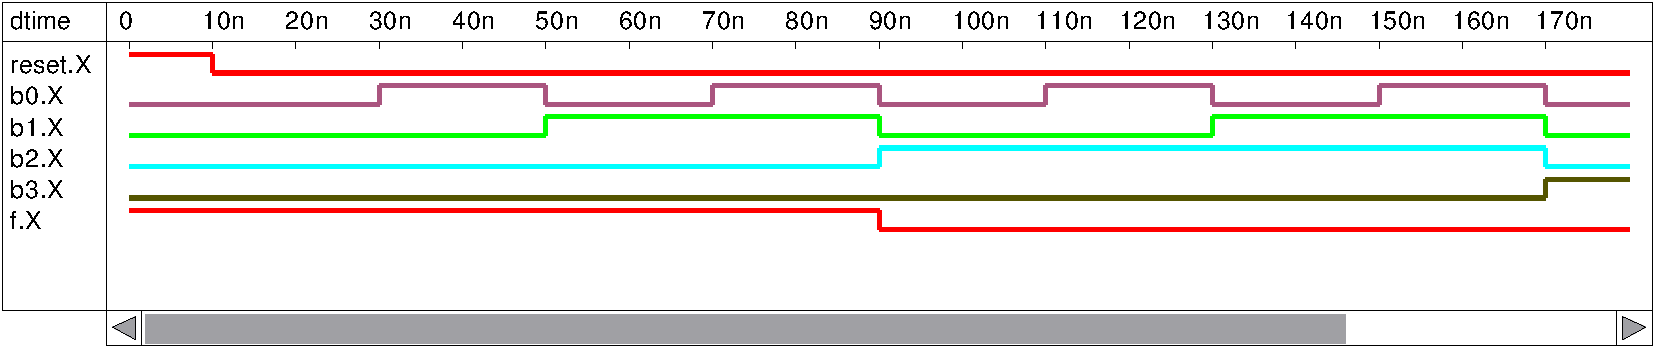
\includegraphics[width=1\linewidth]{dig_ud1_ex2_dpl}
  \caption{Sample simulation waveforms for VHDL editor example 2 design.}
  \label{fig:dig_ud1_ex2_dpl}
\end{figure} 

\item Example 3: VHDL editor example 1 modelled using VHDL process statements and variables.

The VHDL code for the third example is given in the listing at the end
of this paragraph.  In this example the use of VHDL variables is
illustrated.  The VHDL code for the vector generator is a little
unusual in that rather than using the traditional two process design
employing signals, a single process statement employing variables
undertakes both the calculation of the next state data and the
transfer of the next state information to the present state.  This
approach is necessary because FreeHDL does not allowed shared
variables. Once again in this example only single bit data is passed
via the entity statement to the device under test.  The device under
test is represented by a truth table encoded in a process statement.
This is not the most elegant code but it does serve the purpose of
demonstrating the use of different VHDL constructions and data types
in Qucs digital simulation. A typical TimeList plot for VHDL editor
example 3 is shown in Fig.~\ref{fig:dig_ud1_ex3_dpl}.  Comparison of
the three output plots for the VHDL editor examples indicates that all
the simulation results are very similar with some slight differences
in the start up phase following the RESET pulse changing from logic
'1' to logic '0'. This is probably an effect due to the different
initialisation sequences for each of the test vector models.

\begin{lstlisting}[
    language=VHDL,
    basicstyle=\small]
-- Qucs VHDL editor example 3
--
entity test_vector_b is
	port( RESET, CLOCK : in bit;
	      B0, B1, B2, B3 : out  bit
	    );
end entity test_vector_b;
--
architecture behavioural of test_vector_b is
begin
p1 : process(RESET,  CLOCK) is
     variable present_state, next_state :
                bit_vector(3 downto 0):="0000";
          begin	
            if (RESET = '1' ) then next_state := "0000";
            elsif (CLOCK'event and CLOCK='1') then
              present_state := next_state;
            case present_state is
	     when "0000"  =>  next_state := "0001";   
	     when "0001"  =>  next_state := "0010"; 
	     when "0010"  =>  next_state := "0011";  
	     when "0011"  =>  next_state := "0100";   
	     when "0100"  =>  next_state := "0101";   
	     when "0101"  =>  next_state := "0110";   
	     when "0110"  =>  next_state := "0111";   
	     when "0111"  =>  next_state := "1000";   
	     when "1000"  =>  next_state := "1001";   
	     when "1001"  =>  next_state := "1010"; 
	     when "1010"  =>  next_state := "1011"; 
	     when "1011"  =>  next_state := "1100"; 
	     when "1100"  =>  next_state := "1101"; 
	     when "1101"  =>  next_state := "1110"; 
	     when "1110"  =>  next_state := "1111"; 
	     when "1111"  =>  next_state := "0000";
            end case;
            end if;
           B3 <= next_state(3); B2 <= next_state(2); 
           B1 <= next_state(1); B0 <= next_state(0);
        end process p1;
end architecture behavioural;
--
library work;
use work.all;
--
entity testbench is
end entity testbench;
--
architecture dataflow of testbench is  
signal  reset, clk, b0, b1, b2, b3,  f : bit;
begin
p1 : process is
         begin
	    clk <= '0'; wait for 10 ns;
            clk <= '1'; wait for 10 ns;
          end process p1;
--
p2 : process is
        begin
          reset <= '1'; wait for 10 ns;
          reset <= '0'; wait for 2000 ns;
       end process p2;	
--
d1 : entity test_vector_b  port map(reset, clk, b0, b1, b2, b3);
--
--  Behavioural model of combinational circuit
p3: process(b3, b2, b1, b0) is
       variable SEL : bit_vector (3 downto 0);
          begin
            SEL := b3&b2&b1&b0 ;
	    if (SEL = "0010") then f <= '1';
            elsif (SEL = "0000") then f <= '1';
            elsif (SEL = "1111") then f <= '1';
	    elsif (SEL = "0001") then f <= '1';
	    elsif (SEL = "0011") then f <= '1';
            else f <= '0';
            end if;   
      end process p3;
end architecture dataflow;
\end{lstlisting}

\begin{figure}[ht]
  \centering
  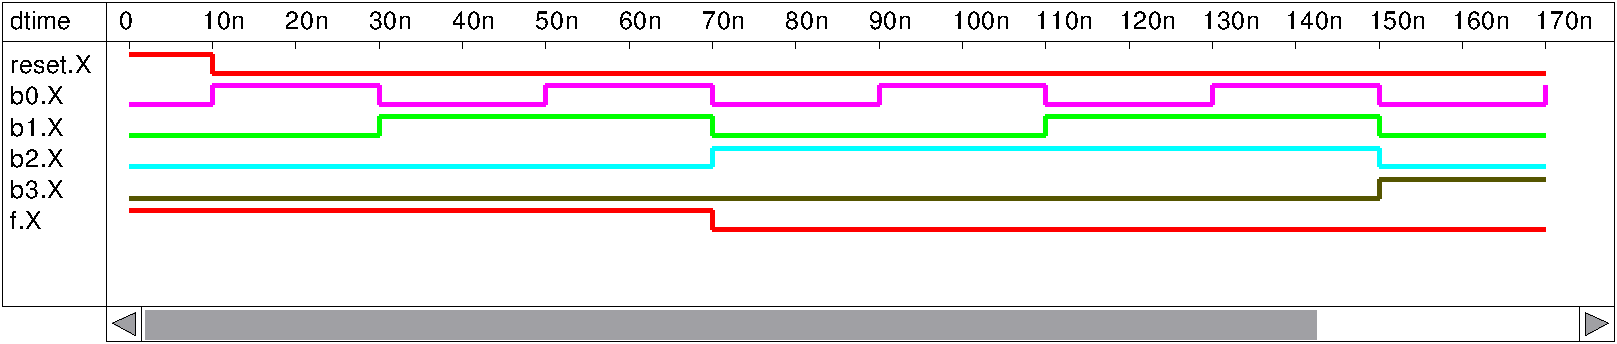
\includegraphics[width=1\linewidth]{dig_ud1_ex3_dpl}
  \caption{Sample simulation waveforms for VHDL editor example 3 design.}
  \label{fig:dig_ud1_ex3_dpl}
\end{figure} 

\end{itemize}

\tutsubsection{Linking VHDL entity-architecture models to Qucs schematic device symbols}

VHDL was originally developed as a hardware description language for
specifying digital systems.  Indeed many engineers still prefer to
describe digital systems entirely in VHDL statements rather than use
schematic drawings.  Once written VHDL code is saved as a text file
and becomes the input data for a VHDL compiler/simulation
package. Through popular demand a number of digital
synthesis/simulator CAD tools\footnote{See for example the XILINX,
WebPACK software at
\url{http//www.xilinx.com/ise/logic_design_prod/webpack.htm}. } have
started to include a facility that links VHDL model code to a
schematic capture symbol. It is then, of course, possible to use a
schematic diagram as the main entry media\footnote{Please note that at
the start of the VHDL simulation process schematic drawings are
converted into a VHDL text file. } when designing and simulating a
digital design.  Qucs release 0.0.9 has such a facility, allowing VHDL
code models to be linked to schematic symbols. When drawing digital
design schematics, these user defined symbols may be mixed with the
Qucs predefined digital symbols and other user defined subcircuit
symbols.  The process for linking VHDL code to Qucs schematic drawing
symbols is straightforward and will be illustrated in these notes
through two examples.

\begin{itemize}
\item Example 4: A 4 bit test vector pattern generator.

Shown in Table~\ref{tab:patgen} is the VHDL entity-architecture model
listing for a 4 bit binary pattern generator.  The VHDL code is
identical to the test vector code introduced in the third VHDL editor
example. After entering the VHDL entity-architecture model code using
the Qucs VHDL editor the finished text is saved in a file with a
suitable name and file extension vhdl. Qucs then lists the model under
the VHDL project category. Simply clicking on a model name in the VHDL
category, with the left hand mouse button, then moving the mouse
pointer to a suitable position on a schematic, causes Qucs to move a
symbol that represents the model onto the schematic drawing
sheet. Placement of the symbol at the position located by the mouse
pointer is achieved by clicking the left hand mouse button. The
procedure is identical to that used to select and place the Qucs
predefined symbols on a schematic drawing. Qucs automatically
generates a rectangular symbol with a name called VHDL that has the
same number of pins as the port statement listed in the VHDL model
entity statement.  Each of the pins is given a name that corresponds
to a name in the entity statement.  Qucs fixes the order of the pins
on the generated symbol.  It appears that it is not possible to edit
this symbol.  However, subcircuit in, out or inout port symbols can be
attached to symbol VHDL and a user edited symbol generated.
Fig.~\ref{fig:dig_ud1_sex1_sch} shows the Qucs generated VHDL symbol
with attached ports for the model listed in Table~\ref{tab:patgen}.
The edited symbol for the 4 bit binary pattern generator is
illustrated in Fig.~\ref{fig:dig_ud1_sex2_sch}.  Notice that in
Fig.~\ref{fig:dig_ud1_sex2_sch} the order of the pins has been changed
to reflect the natural order for a device with it's input pins on the
left and output pins on the right.  VHDL model symbols can also be
generated by placing the VHDL file component, this is located in the
digital components viewlist, on a schematic. On editing the VHDL file
name property of this device to the name of a VHDL entity-architecture
model file, Qucs automatically generates a VHDL symbol. Defining your
own symbol then proceeds in a similar fashion to the way described
above.

\begin{table}
\begin{lstlisting}[
    language=VHDL,
    basicstyle=\small]
entity patgen_4bit is
	port( RESET, CLOCK : in bit;
	        B0, B1, B2, B3 : out  bit
	      );
end entity patgen_4bit;
--
architecture behavioural of patgen_4bit is
begin
p1 : process(RESET,  CLOCK) is
     variable present_state, next_state : 
	       bit_vector(3 downto 0):="0000";
     begin	
      if (RESET = '1' ) then next_state := "0000";
      elsif (CLOCK'event and CLOCK='1') then
      present_state := next_state;
      case present_state is
       when "0000"  =>  next_state := "0001";   
       when "0001"  =>  next_state := "0010"; 
       when "0010"  =>  next_state := "0011";  
       when "0011"  =>  next_state := "0100";   
       when "0100"  =>  next_state := "0101";   
       when "0101"  =>  next_state := "0110";   
       when "0110"  =>  next_state := "0111";   
       when "0111"  =>  next_state := "1000";   
       when "1000"  =>  next_state := "1001";   
       when "1001"  =>  next_state := "1010"; 
       when "1010"  =>  next_state := "1011"; 
       when "1011"  =>  next_state := "1100"; 
       when "1100"  =>  next_state := "1101"; 
       when "1101"  =>  next_state := "1110"; 
       when "1110"  =>  next_state := "1111"; 
       when "1111"  =>  next_state := "0000";
      end case;
      end if;
      B3 <= next_state(3); B2 <= next_state(2); 
      B1 <= next_state(1); B0 <= next_state(0);
     end process p1;
end architecture behavioural;
\end{lstlisting}
\caption{VHDL code for a 4 bit pattern generator.}
\label{tab:patgen}
\end{table}

 \begin{figure}[ht]
  \centering
  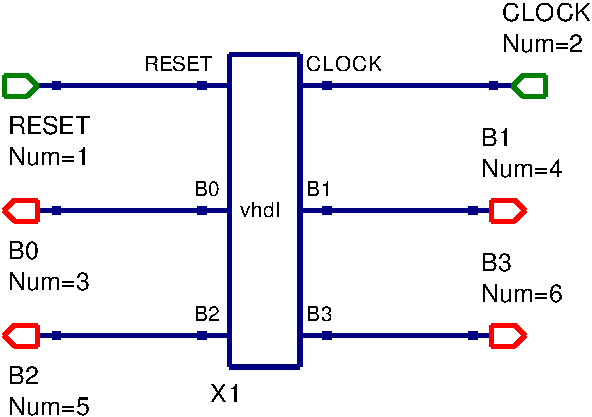
\includegraphics[width=0.6\linewidth]{dig_ud1_sex1_sch}
  \caption{Qucs generated VHDL symbol with subcircuit ports for test pattern generator.}
  \label{fig:dig_ud1_sex1_sch}
\end{figure} 

\begin{figure}[ht]
  \centering
  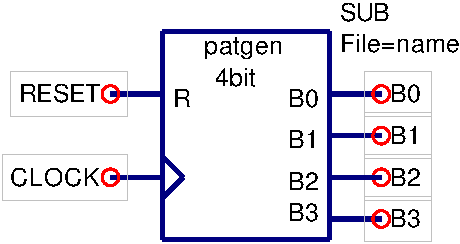
\includegraphics[width=0.5\linewidth]{dig_ud1_sex2_sch}
  \caption{User defined 4 bit pattern generator symbol.}
  \label{fig:dig_ud1_sex2_sch}
\end{figure} 

\item Example 5: A 4 bit full adder.

VHDL model symbols may be combined with either the Qucs predefined
digital component symbols or other subcircuit symbols.  In this
example a VHDL model for a simple one bit full adder is connected four
times in a serial fashion to form a 4 bit full adder.  The VHDL model
code for a simple one bit full adder is given in
Table~\ref{tab:full_adder_1bit}.  The associated symbol diagrams for
the one bit full adder are illustrated in
Fig.~\ref{fig:dig_ud1_sex3_sch} and Fig.~\ref{fig:dig_ud1_sex4_sch}.

\begin{table}
\begin{lstlisting}[
    language=VHDL,
    basicstyle=\small]

--  Full adder - 1 bit
entity fulladder is
	port (a, b, cin : in bit;
	        sum, cout : out bit
	       );
end entity fulladder;
--
architecture dataflow of fulladder is
begin
	sum <= (a xor b) xor cin;
	cout <= (a and b) or (a and cin) or (b and cin);
end architecture dataflow;
\end{lstlisting}
\caption{VHDL code for a 1 bit full adder.}
\label{tab:full_adder_1bit}
\end{table}

 \begin{figure}[ht]
  \centering
  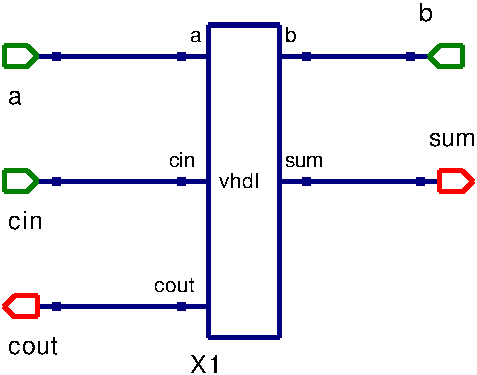
\includegraphics[width=0.6\linewidth]{dig_ud1_sex3_sch}
  \caption{Qucs generated VHDL symbol with subcircuit ports for one bit full adder.}
  \label{fig:dig_ud1_sex3_sch}
\end{figure} 
\FloatBarrier
\begin{figure}[ht]
  \centering
  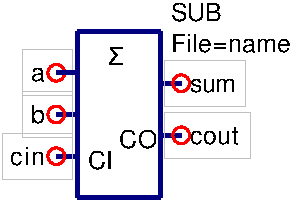
\includegraphics[width=0.4\linewidth]{dig_ud1_sex4_sch}
  \caption{User defined one bit full symbol.}
  \label{fig:dig_ud1_sex4_sch}
\end{figure} 

Figure~\ref{fig:dig_ud1_sex5_sch} shows the schematic for a simple 4
bit ripple adder.  The corresponding user defined symbol for the 4 bit
full adder is given in Fig.~\ref{fig:dig_ud1_sex6_sch}.

\FloatBarrier
\begin{figure}[ht]
  \centering
  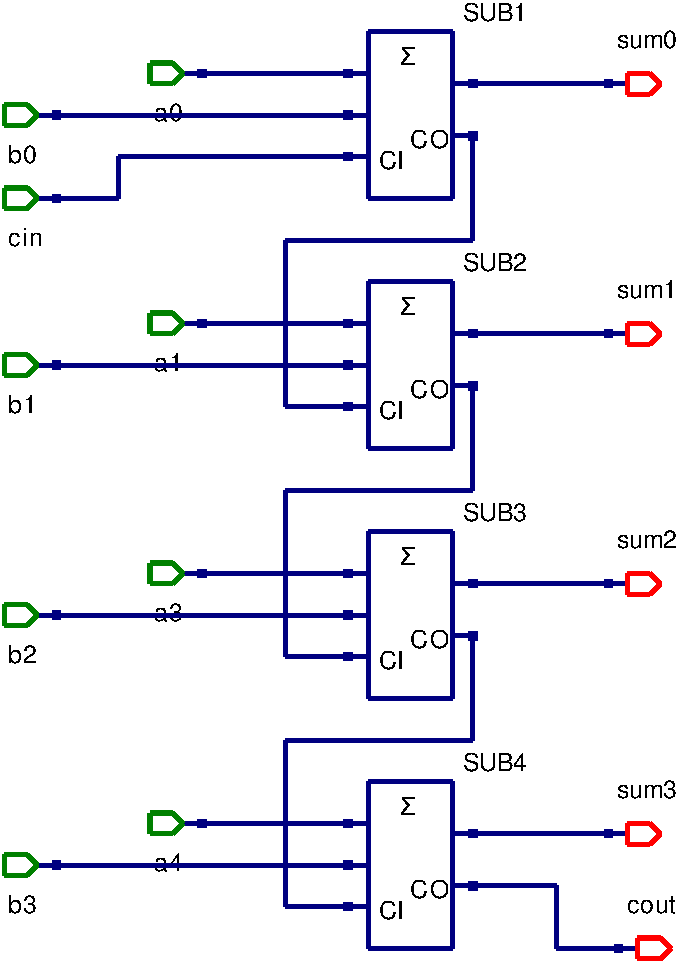
\includegraphics[width=0.4\linewidth]{dig_ud1_sex5_sch}
  \caption{4 bit full adder schematic.}
  \label{fig:dig_ud1_sex5_sch}
\end{figure} 
\FloatBarrier
\begin{figure}[ht]
  \centering
  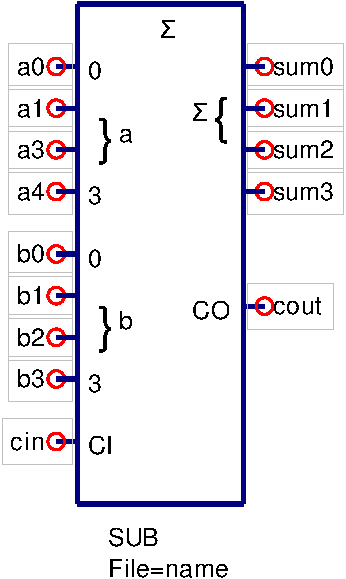
\includegraphics[width=0.3\linewidth]{dig_ud1_sex6_sch}
  \caption{User defined 4 bit full adder symbol.}
  \label{fig:dig_ud1_sex6_sch}
\end{figure} 

 \end{itemize}

\tutsubsection{Generating VHDL code from Qucs schematic drawings}

Pressing key F2 causes Qucs to simulate the design entered by the Qucs
user. The input data for a simulation is either a VHDL text file,
saved from the VHDL text editor, or a VHDL code file generated by Qucs
using the information encoded on a schematic drawing.  In this section
of these tutorial notes a larger design is introduced and the
resulting VHDL code and simulation results are discussed.  The example
chosen for this purpose is a 4 bit by 4 bit combinational digital
multiplier.  Both the 4 bit pattern generator and the 4 bit full adder
outlined in the last section form part of the central core of the 4
bit multiplier design and it's associated testbench.
Table~\ref{tab:mult1} shows the multiplication product table for a 4
bit by 4 bit combinational binary multiplier.  Inputs to the device
are binary bits a3 a2 a1 a0 and b3 b2 b1 b0.  The 4 by 4 multiplier
device requires 16 and gates (to generate the multiplier product
terms), three four bit full adders (to sum the output r terms) and two
4 bit pattern generators to test the 256 possible input states. The
multiplier output is represented in Table~\ref{tab:mult1} by r7 r6 r5
r4 r3 r2 r1 and r0. The circuit schematic for the 4 bit by 4 bit
multiplier and test bench are given in Fig.~\ref{fig:mult_sch}.

\begin{table}
\centering
% use packages: array
\begin{tabular}{llllllll}
 &   &   &   & b3 & b2 & b1 & b0 \\ 
  &   &   &   & a3 & a2 & a1 & a0 \\ 
  &   &   &   & a0b3 & a0b2 & a0b1 & a0b0 \\ 
  &   &   & a1b3 & a1b2 & a1b1 & a1b0 &   \\ 
  &   & a2b3 & a2b2 & a2b1 & a2b0 &   &   \\ 
  & a3b3 & a3b2 & a3b1 & a3b0 &   &   &   \\ 
r7 & r6 & r5 & r4 & r3 & r2 & r1 & r0
\end{tabular}
\caption{Product table for a 4 bit by 4 bit combinational multiplier.}
\label{tab:mult1}
\end{table}

\FloatBarrier
\begin{figure}[ht]
  \centering
  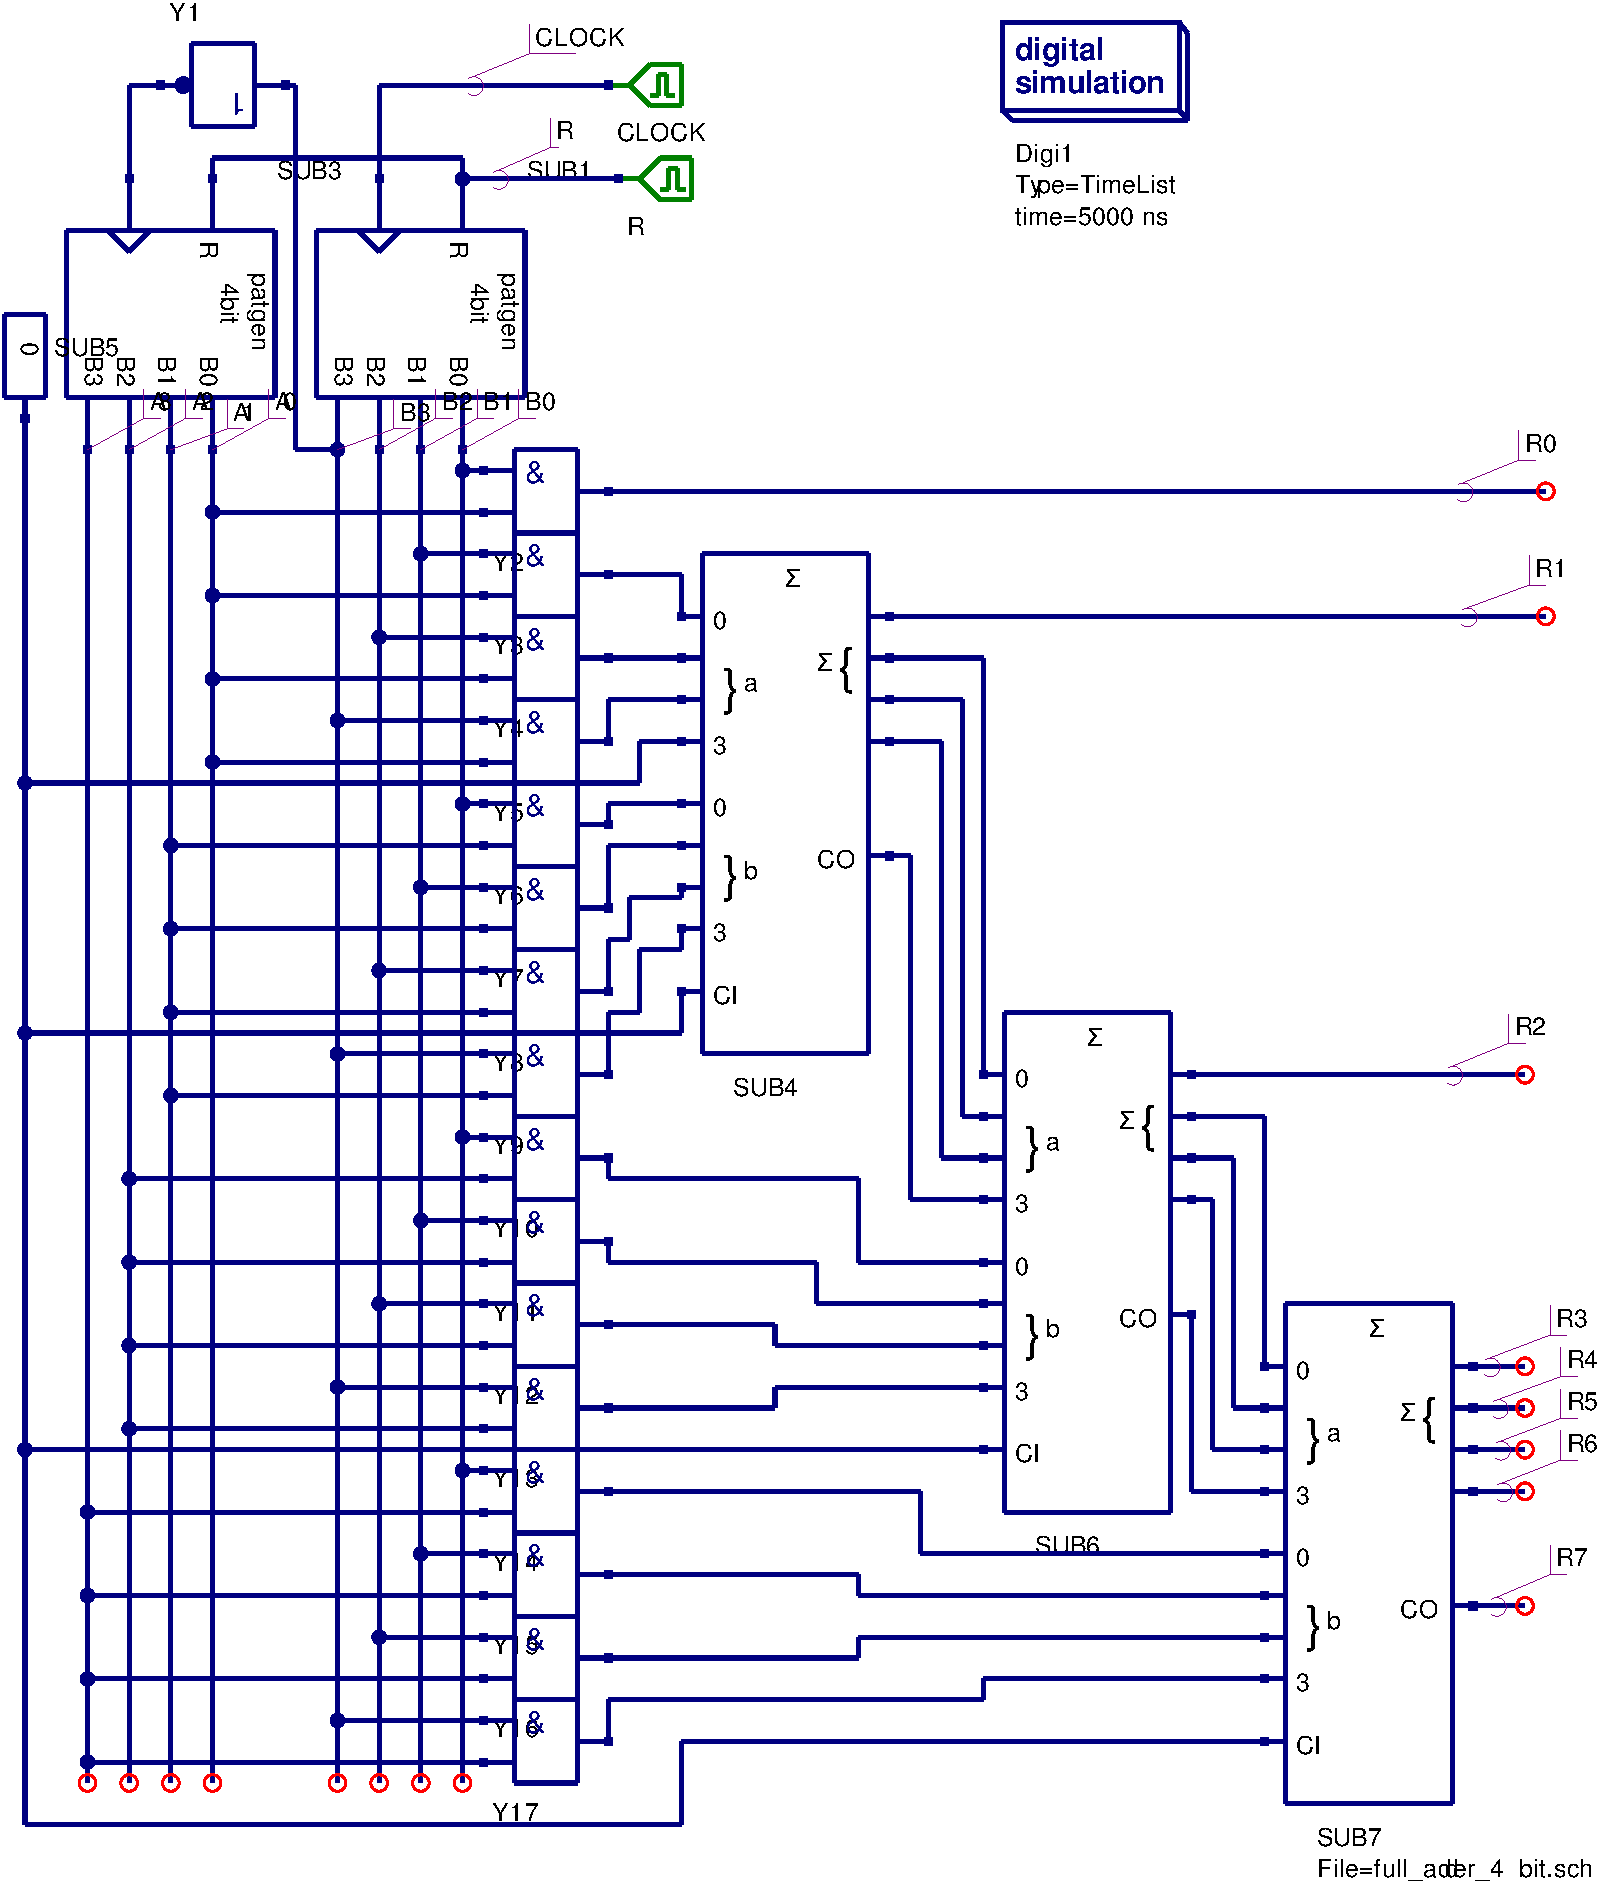
\includegraphics[width=1\linewidth]{mult_sch}
  \caption{A 4 bit by 4 bit combinational digital multiplier.}
  \label{fig:mult_sch}
\end{figure} 

\addvspace{12pt}

The VHDL code for this example is presented in the following listing.
This listing was generated by Qucs\footnote{Some readers will have
noticed that the naming scheme for internal signal nets is different
in the multiplier VHDL listing when compared to the VHDL listings in
the first version of these notes. Towards the end of the 0.0.9
development phase the naming convention employed by Qucs was changed
to give a more flexible structure.}. A small section of the TimeList
waveform plot for the digital multiplier is shown in
Fig.~\ref{fig:mult_dpl}.  At 1.74 micro seconds input a is "0101",
input b is "0111" and the output r is "00100011" which is 35 in
decimal.  Taking a few random checks of the simulation results
indicates that the 4 bit by 4 bit multiplier design works correctly.
Notice that the VHDL code generated by Qucs for the 4 bit multiplier
does not contain any propagation delay timing data.  This could be
added to the and gates, if required.  However, at this stage in the
development of Qucs digital simulation passing timing data, and other
parameters, from device symbols generated from VHDL models has not
been implemented yet. The use of VHDL generics is an obvious way this
could be done. Generics are allowed, of course, in text based VHDL
simulations.

\FloatBarrier
\begin{lstlisting}[
    language=VHDL,
    basicstyle=\small]
-- Qucs 0.0.9  
--  /mnt/hda2/vhdl_comp_lib_prj/multiplier_4bx4bit.sch

entity patgen_4bit is
	port( RESET, CLOCK : in bit;
	        B0, B1, B2, B3 : out  bit
	      );
end entity patgen_4bit;
--
architecture behavioural of patgen_4bit is
begin
 p1 : process(RESET,  CLOCK) is
        variable present_state, next_state : 
             bit_vector(3 downto 0) := "0000";
          begin	
            if (RESET = '1' ) then next_state := "0000";
            elsif (CLOCK'event and CLOCK='1') then
              present_state := next_state;
              case present_state is
	    when "0000" =>  next_state := "0001";   
	    when "0001"  =>  next_state := "0010"; 
	    when "0010"  =>  next_state := "0011";  
	    when "0011"  =>  next_state := "0100";   
	    when "0100"  =>  next_state := "0101";   
	    when "0101"  =>  next_state := "0110";   
	    when "0110"  =>  next_state := "0111";   
	    when "0111"  =>  next_state := "1000";   
	    when "1000"  =>  next_state := "1001";   
	    when "1001"  =>  next_state := "1010"; 
	    when "1010"  =>  next_state := "1011"; 
	    when "1011"  =>  next_state := "1100"; 
	    when "1100"  =>  next_state := "1101"; 
	    when "1101"  =>  next_state := "1110"; 
	    when "1110"  =>  next_state := "1111"; 
	    when "1111"  =>  next_state := "0000";
              end case;
             end if;
           B3 <= next_state(3); B2 <= next_state(2); 
           B1 <= next_state(1); B0 <= next_state(0);
        end process p1;
end architecture behavioural;

entity Sub_patgen_4bit is
  port (net_net0: in bit;
        net_net5: in bit;
        net_outnet_net1: out bit;
        net_outnet_net3: out bit;
        net_outnet_net2: out bit;
        net_outnet_net4: out bit);
end entity;
use work.all;
architecture Arch_Sub_patgen_4bit of Sub_patgen_4bit is
  signal net_net1,
         net_net2,
         net_net3,
         net_net4 : bit;
begin
  net_outnet_net1 <= net_net1 or '0';
  net_outnet_net2 <= net_net2 or '0';
  net_outnet_net3 <= net_net3 or '0';
  net_outnet_net4 <= net_net4 or '0';
  X1: entity patgen_4bit port map (net_net0, net_net5, 
        net_net1, net_net3, net_net2, net_net4);
end architecture;


--  logic_zero.vhdl
entity logic_zero is
	port( Y : out bit
	      );
end entity logic_zero;
--
architecture dataflow of logic_zero is
begin
	Y <= '0';
end architecture  dataflow;


entity Sub_logic_zero is
  port (net_outnetY: out bit);
end entity;
use work.all;
architecture Arch_Sub_logic_zero of Sub_logic_zero is
  signal netY : bit;
begin
  X1: entity logic_zero port map (netY);
  net_outnetY <= netY or '0';
end architecture;


--  Full adder - 1 bit
entity fulladder is
	port (a, b, cin : in bit;
	        sum, cout : out bit
	       );
end entity fulladder;
--
architecture dataflow of fulladder is
begin
	sum <= (a xor b) xor cin;
	cout <= (a and b) or (a and cin) or (b and cin);
end architecture dataflow;


entity Sub_full_adder_1bit is
  port (net_net0: in bit;
        net_net1: in bit;
        net_net2: in bit;
        net_outnet_net3: out bit;
        net_outnet_net4: out bit);
end entity;
use work.all;
architecture Arch_Sub_full_adder_1bit of Sub_full_adder_1bit is
  signal net_net3,
         net_net4 : bit;
begin
  X1: entity fulladder port map (net_net0, net_net1, 
           net_net2, net_net3, net_net4);
  net_outnet_net3 <= net_net3 or '0';
  net_outnet_net4 <= net_net4 or '0';
end architecture;


entity Sub_full_adder_4bit is
  port (net_net0: in bit;
        net_net1: in bit;
        net_net2: in bit;
        net_net3: in bit;
        net_net4: in bit;
        net_net5: in bit;
        net_net6: in bit;
        net_net13: in bit;
        net_net7: in bit;
        net_outnet_net8: out bit;
        net_outnet_net9: out bit;
        net_outnet_net10: out bit;
        net_outnet_net11: out bit;
        net_outnet_net12: out bit);
end entity;
use work.all;
architecture Arch_Sub_full_adder_4bit of Sub_full_adder_4bit is
  signal net_net14,
         net_net15,
         net_net16,
         net_net8,
         net_net9,
         net_net10,
         net_net11,
         net_net12 : bit;
begin
  net_outnet_net8 <= net_net8 or '0';
  net_outnet_net9 <= net_net9 or '0';
  net_outnet_net10 <= net_net10 or '0';
  net_outnet_net11 <= net_net11 or '0';
  net_outnet_net12 <= net_net12 or '0';
  SUB4: entity Sub_full_adder_1bit port map (net_net3, net_net13, 
               net_net14, net_net11, net_net12);
  SUB3: entity Sub_full_adder_1bit port map (net_net2, net_net6, 
               net_net15, net_net10, net_net14);
  SUB2: entity Sub_full_adder_1bit port map (net_net1, net_net5, 
               net_net16, net_net9, net_net15);
  SUB1: entity Sub_full_adder_1bit port map (net_net0, net_net4, 
               net_net7, net_net8, net_net16);
end architecture;

entity TestBench is
end entity;
use work.all;

architecture Arch_TestBench of TestBench is
  signal netA0, netA1, netA2, netA3, netR,  netB0,
         netB1, netB2, netB3, netR0, netR1, netR2,
         netR3, netR4, netR5, netR6, netR7, netCLOCK,
         net_net0, net_net1, net_net2, net_net3, net_net4,
         net_net5, net_net6, net_net7, net_net8, net_net9,
         net_net10,net_net11, net_net12, net_net13, net_net14,
         net_net15, net_net16, net_net17, net_net18, net_net19,
         net_net20, net_net21, net_net22, net_net23,
         net_net24 : bit;
begin
  SUB3: entity Sub_patgen_4bit port map (netR, net_net0, 
              netA0, netA1, netA2, netA3);
  SUB1: entity Sub_patgen_4bit port map (netR, netCLOCK, 
              netB0, netB1, netB2, netB3);

  R:process
  begin
    netR <= '1';  wait for 10 ns;
    netR <= '0';  wait for 2000 ns;
  end process;


  CLOCK:process
  begin
    netCLOCK <= '0';  wait for 10 ns;
    netCLOCK <= '1';  wait for 10 ns;
  end process;

  net_net0 <= not netB3;
  netR0 <= netA0 and netB0;
  net_net1 <= netA0 and netB1;
  net_net2 <= netA0 and netB2;
  net_net3 <= netA0 and netB3;
  SUB5: entity Sub_logic_zero port map (net_net4);
  net_net5 <= netA1 and netB0;
  net_net6 <= netA1 and netB1;
  net_net7 <= netA1 and netB2;
  net_net8 <= netA1 and netB3;
  net_net9 <= netA2 and netB0;
  net_net10 <= netA2 and netB1;
  net_net11 <= netA2 and netB2;
  net_net12 <= netA2 and netB3;
  SUB4: entity Sub_full_adder_4bit port map (net_net1, net_net2, 
               net_net3, net_net4, net_net5, net_net6, net_net7, 
               net_net8, net_net4, netR1, net_net13, net_net14, 
               net_net15, net_net16);
  SUB6: entity Sub_full_adder_4bit port map (net_net13, net_net14, 
               net_net15, net_net16, net_net9, net_net10, net_net11, 
               net_net12, net_net4, netR2, net_net17, net_net18, 
               net_net19, net_net20);
  net_net21 <= netA3 and netB0;
  net_net22 <= netA3 and netB1;
  net_net23 <= netA3 and netB2;
  net_net24 <= netA3 and netB3;
  SUB7: entity Sub_full_adder_4bit port map (net_net17, net_net18, 
               net_net19, net_net20, net_net21, net_net22, 
               net_net23, net_net24, net_net4, netR3, netR4, 
               netR5, netR6, netR7);
end architecture;
\end{lstlisting}

\begin{figure}[ht]
  \centering
  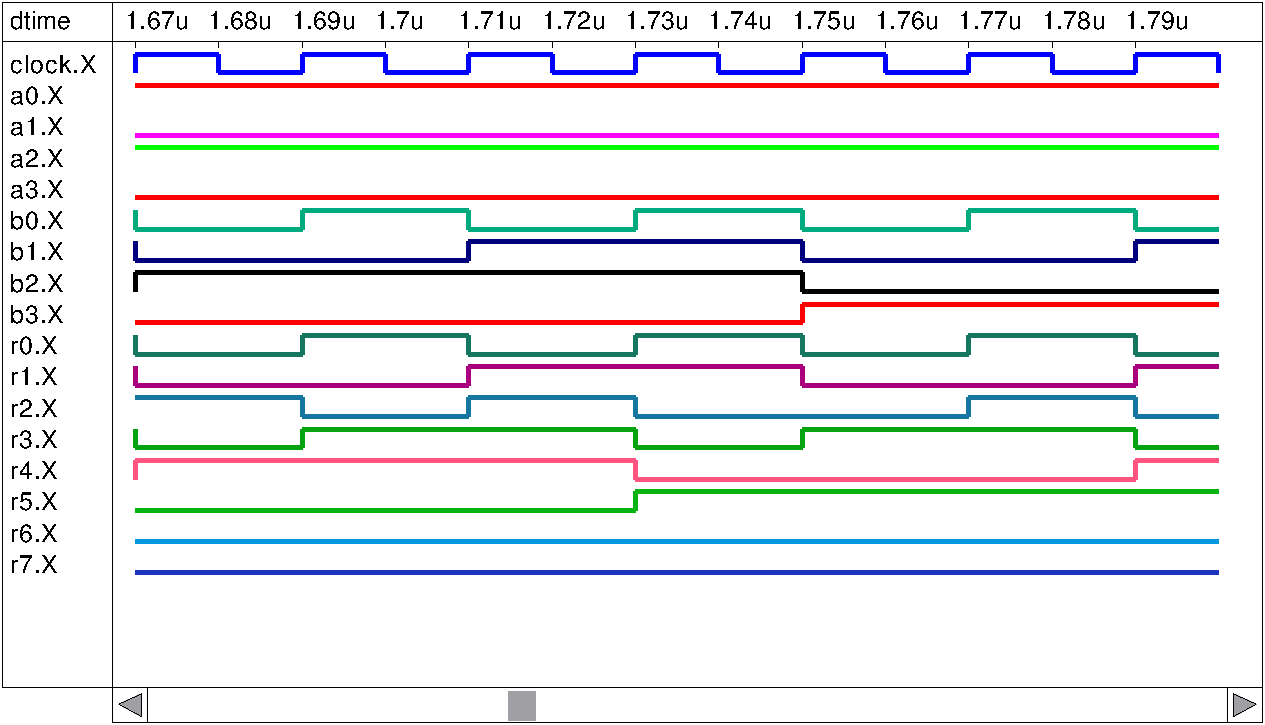
\includegraphics[width=1\linewidth]{mult_dpl}
  \caption{A section of the 4 bit by 4 bit combinational digital multiplier TimeList output waveforms.}
  \label{fig:mult_dpl}
\end{figure} 

\tutsection{Update number two: September 2006}

Update number two in this tutorial series reports on the major changes that have taken place to Qucs digital simulation since the first update was posted on the Qucs Web site roughly three months ago.  During this period a number of significant, and very critical, extensions have been implemented. Previous releases concentrated on establishing a fundamental base for digital circuit simulation using the VHDL language. The primary vehicle for representing circuit signals being the VHDL bit and bit-vector signal types. The next release of Qucs (version 0.0.10) and FreeHDL (version 0.0.3) extends the allowed signal types to include \verb|IEEE std_logic_1164| nine level logic, integers, and reals. Readers will appreciate that these changes are the result of a great deal of work by the Qucs team and must be considered as very much work in progress because not all the features offered by the FreeHDL implementation of the VHDL language are currently available via the Qucs schematic capture and VHDL text file simulation routes. Although a significant amount of testing has taken place it is likely that software bugs will come to light as more Qucs users try the new features - if you find a bug please report it by posting a note on the Qucs Web site. Adding new signal types to Qucs digital simulation affects all sections of the simulation route from schematic capture to plotting and tabulating input and output signals.  Hence, although it may seem the wrong way round, the place to first implement the necessary changes to accommodate the new signal types is at the simulation results reporting stages of the Qucs package.  In release 0.0.10 no attempt has been made to add the new signal types to the schematic capture part of the Qucs package.\footnote{Adding new signal types to Qucs schematic capture is on the to-do list.}   Recent work on the digital sections of the Qucs package has concentrated on (1) improvements to VHDL language entry using the Qucs colour coded VHDL text editor\footnote{A number of editor bugs have been fixed and it is now possible for users to define their own colour scheme for the various classes of VHDL reserved words and data types.}, (2) modifications to FreeHDL which allow a cleaner interface between Qucs and FreeHDL, (3) upgrades to the data conversion of simulation results from the FreeHDL value change dump format to the native Qucs format, and (4) major changes to the results reporting routines that are accessed from the Qucs diagrams icon dialogue.  A detailed list of the software changes and bug fixes can be found in the Qucs and FreeHDL change log files.


\tutsubsection{Simulating VHDL code using Qucs and FreeHDL.}

The flow diagram drawn in Fig.~\ref{fig:digital_ud1_fa} shows the relationship between Qucs and FreeHDL, and the sequence that takes place during digital circuit simulation.  This flow diagram does not however, outline the details of the stages that are performed when converting (1) VHDL circuit code into a machine code simulation program, and (2) simulation output results into a format that can be plotted and tabulated by Qucs.  These are illustrated in the flow diagram presented in Fig.~\ref{fig:ud2_fig1}.   The shell script qucsdigi controls each of the stages in this sequence.  A basic understanding of the process employed by Qucs and FreeHDL is needed if users of the software are to be able to write meaningful VHDL code and simulate it using the two packages.  VHDL code is either generated from a schematic diagram automatically by Qucs or entered using the Qucs VHDL text editor.  The use of the schematic entry route was described in update one of these tutorial notes.  However, a number of readers will probably have spotted that included in the VHDL code generated by Qucs are references to VHDL libraries.  The VHDL language uses libraries to provide features that are not specified in the basic language definition but are commonly used by all language processing systems; two such libraries are STD and IEEE.  When simulating digital circuits a basic knowledge of the structure of a simulation task and how these employ VHDL libraries is essential.  This implies that users of the Qucs/FreeHDL software must appreciate how the system compiles and simulates a VHDL circuit simulation task.  Once the VHDL simulation code has been entered via the VHDL text editor clicking the Qucs simulation button runs shell script qucsdigi performing the sequence shown in Fig.~\ref{fig:ud2_fig1}\footnote{For the FreeHDL package to operate correctly the directory where the software is installed must be included in the shell PATH from which Qucs is launched.}. Program freeehdl-v2cc converts VHDL code into C++ functions.  These are then compiled along with a main C++ function.  The next stage in the sequence links the compiled object code with the object code from any references to items in the predefined VHDL libraries to produce an executable digital simulation program.  This is then run by Qucs outputting a set of simulation results in value change dump (VCD) format\footnote{The value change dump language was originally designed as a simulation waveform interchange format for Verilog HDL. The specification of the VCD format can be found at http://www-ee.eng.hawaii.edu/~msmith/ASICs/HTML/Verilog/LRM/HTML/15/ch15.2.htm }. Finally a program called qucsconv converts the VCD simulation results into the Qucs native data format ready for post processing as graphical or tabular diagrams by Qucs.

\FloatBarrier
\begin{figure}[ht]
  \centering
  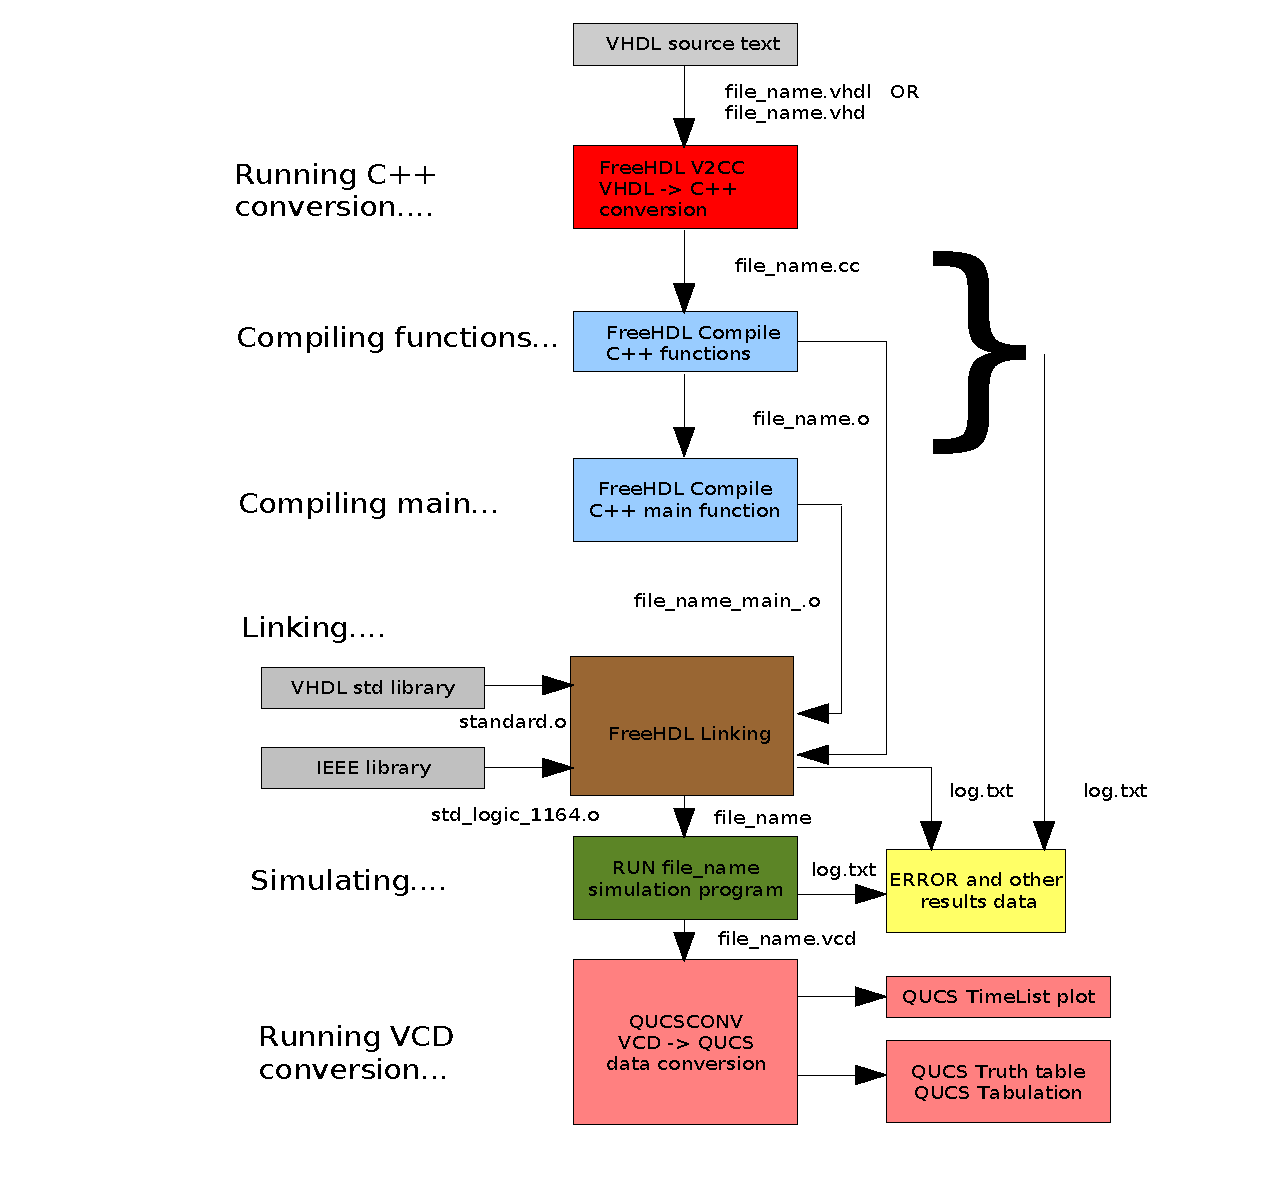
\includegraphics[width=1.0\linewidth]{dig_ud2_fig1} 
  \caption{Detailed flow diagram showing VHDL code compilation and simulation results processing.}
  \label{fig:ud2_fig1}
\end{figure} 
\FloatBarrier


\tutsubsection{VHDL predefined packages and libraries.}

All VHDL language processing systems provide a predefined VHDL package called standard.  This package defines many of the fundamental VHDL data types, for example bit, character, integer and real. The predefined types, subtypes and other functions in the package standard are stored in a library called STD. The FreeHDL version of library STD includes an additional VHDL package called textio which is used to input and output signal data from and to files.  A second library called IEEE defines (1) multivalued logic signals defined by nine different encoding values, making it possible to model digital circuits that are composed from different technology components, (2) logic signal subtypes and (3) an extensive range of useful functions, procedures and overloaded operators.  The FreeHDL version of the IEEE library consists of the following packages:
\begin{enumerate}
\item \verb|std_logic_1164|
\item \verb|numeric_bit|
\item \verb|math_real|
\item \verb|numeric_std|
\item \verb|std_logic_arith|
\item \verb|std_logic_unsigned|
\item \verb|vital_timing|
\end{enumerate}

One other library is always defined by VHDL code processing systems namely the work library.  This library holds user compiled VHDL entity/architecture design units.

\tutsubsection{VHDL simulation code structures.}

In its most basic form VHDL circuit simulation code is structured as an entity-architecture test bench which includes input signal test information.\footnote{Test signals are often called test vectors.} An example outline of the basic format is 

\begin{lstlisting}[
    language=VHDL,
    basicstyle=\small]
entity testbench is
--  entity body statements
end entity testbench;
--
architecture behavioural of testbench is
--  architecture body statements
end architecture behavioural;
\end{lstlisting}

VHDL data types, functions and operators in package standard are always visible to VHDL test bench code and reference to their use need not be added explicitly. However, if the test bench entity-architecture uses data types or other items defined in other libraries, for example the \verb|std_logic| type in the IEEE library, then reference to them needs to be added before each entity-architecture pair where they are used.  Libraries are referenced using the VHDL \textit{library} and \textit{use} statements.  An example showing how these statements are employed is outlined in the following VHDL code segment:
  
\begin{lstlisting}[
    language=VHDL,
    basicstyle=\small]
library ieee;
use ieee.std_logic_1164.all;
--
entity testbench is
--  entity body statements
end entity testbench;
--
architecture behavioural of testbench is
--  architecture body statements
end architecture behavioural;
\end{lstlisting}

Here the VHDL code word \textit{all} signifies that all items in a specific library are to be made available for use in the following entity/architecture pair; testbench in the above example.  If more than one library is to be used then a library/use statement is needed for each library reference.  Most complete VHDL circuit simulation programs consist of more than one entity/architecture pair.  In such cases the circuit test bench, with its signal test vectors, must be the last entry in the program.  An example of a more complex VHDL program structure is

\begin{lstlisting}[
    language=VHDL,
    basicstyle=\small]
library ieee;
use ieee.std_logic_1164.all;
--
entity comp1 is
--  entity body statements
end entity comp1;
--
architecture behavioural of comp1 is
--  architecture body statements
end architecture behavioural;
--
library ieee;
use ieee.std_logic_1164.all;
--
entity comp2 is
--  entity body statements
end entity comp2;
--
architecture behavioural of comp2 is
--  architecture body statements
end architecture behavioural;

--
library ieee;
use ieee.std_logic_1164.all;
--
use work.all;
--
entity testbench is
--  entity body statements
end entity testbench;
--
architecture behavioural of testbench is
--  architecture body statements
end architecture behavioural;
 \end{lstlisting}

During the conversion of VHDL code to a machine code simulation program each  entity/architecture pair, prior to the final test bench entry, is compiled as a separate design unit and stored in the work library\footnote{The testbench entity/architecture pair is also, of course, compiled but this design unit is the one that is run as the executable simulation program.}.  Compiled design units held in the work library can be referenced in other entity/architecture models provided the VHDL statement  \textit{use work.all;}\footnote{References to individual items are also allowed by inserting, for example, \textit{use.work.comb1; use.work.comb2;} in the VHDL code.} is inserted in the VHDL simulation code prior to each entity/architecture statement where they are referenced.
\newpage 
\tutsubsection{VHDL data types.} 


\FloatBarrier 
\begin{figure}[ht] 
  \centering 
  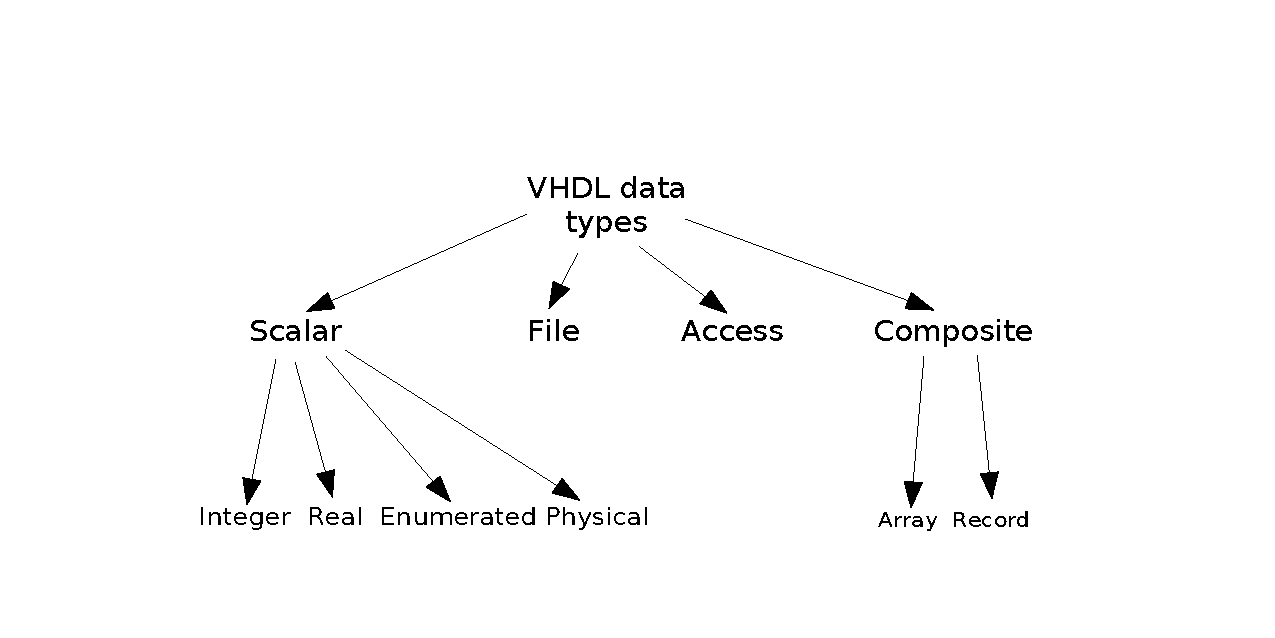
\includegraphics[width=1.0\linewidth]{dig_ud2_fig2} 
  \caption{VHDL data types} 
  \label{fig:ud2_fig2}
\end{figure} 
\FloatBarrier

The chart shown in Fig.~\ref{fig:ud2_fig2} indicates the different data types that are available in the VHDL language. FreeHDL implements all these data types. In practical circuit simulation the different VHDL data types are normally used to specify (1) signals, (2) variables and (3) constants\footnote{Type file is of course different in that it is used to store either test vectors, component data such as ROM contents and output simulation results.}. During simulation Qucs/FreeHDL automatically stores the values of integer, real and enumerated bit signals as simulation time progresses.  Furthermore, \verb|bit_vector| and IEEE signal types including \verb|std_logic_vector| are also stored.  Signals of these types are then available for plotting and tabulation using the Timing, Truth table, Tabular and Cartesian output diagrams.  Selected elements in user defined composite signals, those that are stored in arrays for example\footnote{Please note that signal types based on the composite type record will probably cause the Qucs simulation cycle to fail - work on this data type has been added to the to-do list.}, can be assigned to the basic signal types then displayed.\footnote{Qucs/FreeHDL also automatically collects waveform data for composite signals based on arrays of bit and IEEE signal types. However, in the case of large arrays care is needed when plotting or tabulating these directly because the entire contents of an array is output each time a signal is displayed.}. An example of how this is done is given in later sections of these update tutorial notes. Note - the values of variables and constants are not recorded during simulation.


\tutsubsection{An example VHDL simulation employing integer signals.} 

The following VHDL code demonstrates how the integer data type can be used to represent signals.   In this example signals A, B  change state on the rising edge of clock clk. The code tests the addition of integer signals and constants using arithmetic operators defined in library STD.\footnote{The specification for the FreeHDL library STD can be found in text file freehdl-0.0.3/std/standard.vhdl.} The results from this simulation are shown in Fig.~\ref{fig:ud2_fig3}.

\begin{lstlisting}[
    language=VHDL,
    basicstyle=\small]
-- A very basic test of data type integer.
entity testbench is
end entity testbench;
--
architecture behavioural of testbench is
signal A, B, C :  integer := 0;
signal clk : bit;
begin
p0 : process is  -- Generate clock signal.
        begin
           clk <= '0';   wait for 10 ns;
           clk <= '1';   wait for 10 ns;
       end process p0;
--
p1 : process (clk) is
       begin
         if (clk'event and clk='1') then
           A <= A + 1;
           B <= B + 2;
         end if;
       end process p1;
           C <= A + B ;
end architecture behavioural;
 \end{lstlisting}

\begin{figure}[ht] 
  \centering 
  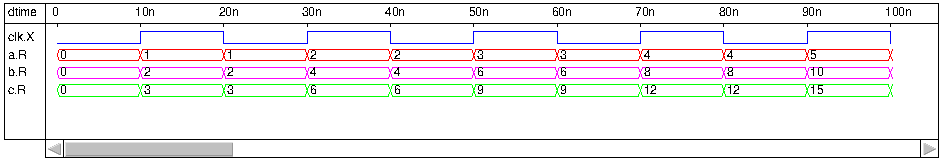
\includegraphics[width=1.0\linewidth]{dig_ud2_fig3} 
  \caption{Output results for a simple test bench example employing integer signals.} 
  \label{fig:ud2_fig3} 
\end{figure} 

\tutsubsection{Multivalued logic.} 

Although signal types bit and bit-vector are widely employed when simulating digital systems one of their great weaknesses is the fact that it is difficult to represent signal bus systems simply using only logic '0' and logic '1' signal encoding.  Moreover, circuits where bus signal contention occurs often result in simulation failure.  The IEEE \verb|std_logic_1164| package overcomes this limitation through the introduction of a multivalued logic system which defines nine different logic values to represent signal types and signal strengths.  Not only is the bus contention problem solved through logic resolving functions but the multivalued logic system allows devices constructed from different manufacturing technologies to be simulated at the same time, ensuring that the simulation process mirrors real circuit design practices.  The next two simulation examples introduce the nine value logic system and demonstrate it's use in the design of digital bus systems. Signals of type real are also introduced to show their representation by Qucs. Listed below is the VHDL code for a basic simulation which generates a set of IEEE \verb|std_logic|, integer and real signals.  Figure~\ref{fig:ud2_fig4} illustrates how the Qucs Timing diagram displays different signal types.  A section of tabulated results are also given in Fig.~\ref{fig:ud2_fig5}.

\begin{lstlisting}[
    language=VHDL,
    basicstyle=\small]

library ieee;
use ieee.std_logic_1164.all;
--
entity testbench is
end entity testbench;
--
architecture behavioural of testbench is
signal clk : bit;
signal bv1 : bit_vector(8 downto 0);
signal stdl1 : std_logic_vector(8 downto 0);
signal INT1 : integer := 0;
signal INT2 : integer := 99;
signal R1 : real := 0.33;
signal R2 : real := 99.0;
signal R3 : real := 0.0;
signal R4 : real := 0.0;
begin
p0 : process is
      begin
	clk <= '0'; wait for 10 ns;
	clk <= '1'; wait for 10 ns;
      end process p0;
--
p1 : process(clk) is
	variable  v1 :  integer := 0;
      	begin
	  if (clk'event and clk = '1') then
		v1 := v1+1;
		case v1 is
		  when 1 => bv1 <= "000000000"; stdl1 <= "000000000";
	          when 2 => bv1 <= "000000001"; stdl1 <= "000000001";
		  when 3 => bv1 <= "000000011"; stdl1 <= "00000001X";
	          when 4 => bv1 <= "000000111"; stdl1 <= "0000001XZ";
		  when 5 => bv1 <= "000001111"; stdl1 <= "000001XZU";
	          when 6 => bv1 <= "000011111"; stdl1 <= "00001XZUW";
		  when 7 => bv1 <= "000111111"; stdl1 <= "0001XZUWL";
	          when 8 => bv1 <= "001111111"; stdl1 <= "001XZUWLH";
                  when 9 => bv1 <= "111111111"; stdl1 <= "01XZUWLH-";
		  when others => v1 := 0;
		end case;
	end if;
          end process p1;
p3 : process (clk) is
        begin
          if (clk'event and clk='1')  then
              INT1 <= INT1 + 1;
	      INT2 <= INT2 -20;
          end if;
--
          if(INT1 >= 9) then
              INT1 <= 0;
              INT2 <= 99;
         end if;
       end process p3;
--
p4 : process (clk) is
         Variable V2 : real;
        begin
          if (clk'event and clk='1')  then
              R1 <= R1 + 1.0;
	      R2 <= R2 -20.0;
              R3 <= R1*R2;
              R4 <= R2/(R1+0.0001);
          end if;
--
          if(R1 >= 20.0) then
              R1 <= 0.0;
              R2 <= 99.0; 
         end if;
       end process p4;
end architecture behavioural;
 \end{lstlisting} 
 
\begin{figure}[ht]   
  \centering 
  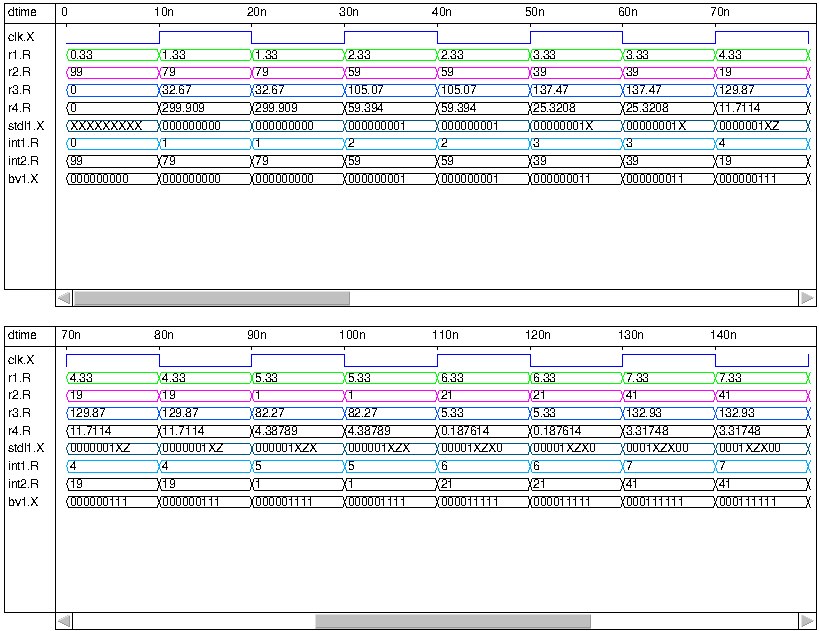
\includegraphics[width=1.1\linewidth]{dig_ud2_fig4} 
  \caption{Output results illustrating the TimeList representation of signals.} 
  \label{fig:ud2_fig4} 
\end{figure} 

\FloatBarrier  
\begin{figure}[ht]   
  \centering 
  \includegraphics[width=1.0\linewidth]{dig_ud2_fig5} 
  \caption{Output results illustrating tabular representation of signals.} 
  \label{fig:ud2_fig5} 
\end{figure} 


\begin{table}
\centering
\begin{center}
% use packages: array
\begin{tabular}{ll}
\textbf{VHDL signal levels} & \textbf{VCD } \\ 
'0'   Forcing logic 0 &    '0'\\ 
'1'   Forcing logic 1 &       '1' \\  
'X'   Forcing unknown &       'X' \\ 
'Z'   High impedance & 'Z' \\ 
'U'   Uninitialised & 'X' \\ 
'W'  Weak unknown & '0' \\ 
'L'   Weak logic 0 & '0' \\ 
'H"  Weak logic 1 & '1' \\ 
'-'    Don't care &  'X'
\end{tabular}
\end{center}

\caption{IEEE multivalue logic and VCD representation.}
\label{tab:tab7}
\end{table}






The VCD waveform interchange standard encodes digital signals as four different logic levels.  These are '0', '1', 'Z' (high impedance) and 'X' (unknown).  Table~\ref{tab:tab7} lists how the nine \verb|ieee.std_logic| signal levels are represented using the VCD format.  Until the VCD standard is revised the Qucs/FreeHDL package is restricted to displaying simulation output data using the basic '0', '1', 'Z' and 'X' signal encoding.  The next example shows how the IEEE \verb|std_logic| signal type can be used to simulate bus logic.  The demonstration has been kept simple in order to keep the VHDL code short. The  code fragment simulates two tri-state buffers which pass their outputs to bus drivers who's outputs connect on a common signal bus.  The bus drivers ensure that the outputs from the tri-state buffers are kept separate before combining onto the common bus line.  This allows the output signals from the tri-state buffers and the combined signal to be plotted separately.  The resulting waveforms clearly show the \verb|std_logic| resolution function in operation, see Fig.~\ref{fig:ud2_fig6} .  Note the effect of the 7 ns delay on the plotted waveforms and the use of the VHDL generic statement to set the invert device delay value.

\begin{lstlisting}[
    language=VHDL,
    basicstyle=\small]

-- Demonstration of a simple bus structure using 
-- the IEEE std_logic data type.
library ieee; 
use ieee.std_logic_1164.all;
--
entity buf  is
        generic(delay : time := 0 ns);
	port (in1, control  : in std_logic;
	      out1 : out std_logic
                    );
end entity buf;
architecture behavioural of buf is
begin
p0 : process (in1, control) is
        begin
          if (control = '1') then out1 <= in1 after delay;
          else out1 <= 'Z';
         end if;
       end process p0;
end architecture behavioural;
--
library ieee;
use ieee.std_logic_1164.all;
--
entity invert is
        generic(delay : time := 0 ns);
	port (in1 : in std_logic;
	      out1 : out std_logic
                   );
end entity invert;
--
architecture behavioural of invert is
begin
   out1 <=  not in1 after delay;
end architecture behavioural;
--
library ieee;
use ieee.std_logic_1164.all;
--

entity buf2 is
  port (in1 : in std_logic;
          out1 : out std_logic
         );
end entity buf2;
--
architecture dataflow of buf2 is
begin
  out1 <= in1;
end architecture dataflow;
--
library ieee;
use ieee.std_logic_1164.all;
--
use work.all;
--
entity testbench is
end entity testbench;
--
architecture structural of testbench is
signal data_in_1, data_in_2 : std_logic;
signal data_out_1,  data_out_2 : std_logic;
signal data_control,  control_buf1 : std_logic;
signal result : std_logic;
--
begin
p0 : process is
       begin
         data_in_1 <= '0'; wait for 5 ns;
         data_in_1 <= '1'; wait for 5 ns;
      end process p0;
--
      data_in_2 <= not data_in_1;
--
p1 : process is
       begin
         data_control <= '1'; wait for 40 ns;
         data_control <= '0'; wait for 40 ns;
      end process p1;
--
c1g1 : entity buf     port map(in1 => data_in_1, control => data_control, 
                               out1 => data_out_1);
c1g2 : entity invert  generic map (delay => 7 ns) 
                      port map(in1 => data_control,out1 => control_buf1);
c1g3 : entity buf     port map(in1 => data_in_2, control => control_buf1, 
                               out1 => data_out_2);
c1g4 : entity  buf2   port map(in1 => data_out_1, out1 => result);
c1g5 : entity  buf2   port map(in1 => data_out_2, out1 => result);
--
end architecture structural;
 \end{lstlisting} 

\FloatBarrier  
\begin{figure}[ht]   
  \centering 
  \includegraphics[width=1.0\linewidth]{dig_ud2_fig6} 
  \caption{Signal waveforms for the simple bus example.} 
  \label{fig:ud2_fig6} 
\end{figure} 

\tutsubsection{Run debugging of VHDL simulation code.} 
The VHDL language has a number of built in features that allow the debugging of VHDL code at simulation time.  In this section the VHDL reserved words \textit{assert, report} and \textit{severity} are introduced and their use as code debugging aids explained by way of a more detailed design example. In the previous digital tutorial update a structural design of a 4 bit digital multiplier was introduced as an example that employed the Qucs schematic capture digital simulation route. The next example extends the previous multiplier design to 16 bits.  However, at a structural level the larger multiplier becomes very detailed and it's design can be prone to error.  To demonstrate the power of VHDL the 16 bit multiplier has been redesigned at a functional level.  A block diagram of the multiplier simulation test bench is given in Fig.~\ref{fig:ud2_fig7}: firstly a clock strobes a data generator unit which generates a sequence of integer numbers. These are converted to 16 \verb|bit_vectors| and applied to the 16 bit multiplier unit as inputs x and y; secondly the 16-bit multiplier on sensing a change in inputs x or y converts these signals from 16 \verb|bit_vectors| to integers, multiples them and finally converts the integer result to 32 \verb|bit_vector| output \verb|Res_bit|. Although standard library STD defines arithmetic operations for integers it does not provide functions for the conversion of integers to \verb|bit_vectors| or the reverse operation. The following VHDL listing gives the complete simulation test bench program for the 16 bit multiplier including the required data conversion functions. VHDL debug or message reporting code using the reserved words assert, report and severity have been added to the \verb|data_generator| and \verb|functional_multiplier| architecture code. During simulation these text strings, and the simulation time when they were actioned, are written to the Qucs log.txt file, giving a trace record of the simulation activity. In cases where an error occurs at severity level failure the simulation will terminate. FreeHDL allows VHDL report statements without an accompanying assert statement.\footnote{One of the changes at the 1993 revision of the IEEE VHDL 1076-1987 standard was to allow report statements without the previous mandatory assert clause.  FreeHDL attempts to comply with the 1993 revision.}  A typical Timing diagram plot for this design is shown in Fig.~\ref{fig:ud2_fig8} 

\FloatBarrier  
\begin{figure}[ht]   
  \centering 
  \includegraphics[width=1.0\linewidth]{dig_ud2_fig7}  
  \caption{Block diagram of a 16 bit functional multiplier.} 
  \label{fig:ud2_fig7} 
\end{figure} 


\begin{lstlisting}[
    language=VHDL,
    basicstyle=\small]
-- 16 bit digital multiplier example.
-- Simulation trace using assert, report and severity statements.
--
entity clock is
    port( clk : out bit);
end entity clock;
--
architecture behavioural of clock is
begin
p0 : process  is
        begin
           clk <= '0' ; wait for 10 ns;
           clk <= '1' ; wait for 10 ns;
       end process p0;
end architecture behavioural;
--
entity data_generator is
     port( clk : in bit;
             x, y : out bit_vector(15 downto 0)
            );
end entity data_generator;
--
architecture behavioural of data_generator is
type mem_array_16  is array(1 to 8) of integer;
signal count : integer := 0;
--
function integer_to_vector_16(int_no : integer) return bit_vector  is
variable ni : integer;
variable return_value : bit_vector(15 downto 0);
begin
   assert (ni < 0)
      report "Function integer_to_vector_32: integer number must be >= 0"
      severity failure;
   ni := int_no;
   for i in return_value'Reverse_Range loop 
      if ( (ni mod 2 ) =1 ) then return_value(i) := '1';
      else return_value(i) := '0';
      end if ;
      ni := ni/2;
   end loop;
   return return_value;
end integer_to_vector_16;
--
begin
p1 : process(clk) is
        variable xi : mem_array_16 := (1, 2, 3, 4, 5, 6, 7, 8);
        variable yi : mem_array_16 := (2, 4, 6, 8, 10, 12, 14, 16);
        variable xh, yh : integer;
        variable counti : integer;
      begin

	counti := count+1;
            if (counti > 8 ) then
                counti := 1;
            end if;
               xh := xi(counti);
               yh := yi(counti);
               x <= integer_to_vector_16(xh);
               y <= integer_to_vector_16(yh);             
               count <= counti;
               report "In process p1.data_generator.";
      end process p1;
end architecture behavioural;
--
--
entity functional_multiplier is
     port(  x, y : in bit_vector(15 downto 0);
             res_bit : out bit_vector(31 downto 0)
            );
end entity functional_multiplier;
--
--
architecture behavioural of functional_multiplier is
--
function vector_to_integer(v1 : bit_vector)  return integer is
variable return_value : integer :=0;
alias v2 : bit_vector(v1'length-1 downto 0) is v1;
begin
   for i in v2'high downto 1 loop
      if (v2(i) = '1') then
               return_value := (return_value+1)*2;
      else
               return_value := return_value*2;
     end if;
   end loop;
   if v2(0) = '1' then return_value:= return_value+1;
   end if;
return return_value;
end vector_to_integer;
--
function integer_to_vector_32(int_no : integer) return bit_vector  is
variable ni : integer;
variable value : bit_vector(31 downto 0);
begin
   assert (ni < 0)
      report "Function integer_to_vector_32: integer number must be >= 0"
      severity failure;
   ni := int_no;
   for i in 0 to 31 loop 
      if ( (ni mod 2 ) =1 ) then value(i) := '1';
      else value(i) := '0';
      end if ;
      if ni > 0 then ni := ni/2;
      else ni := (ni-1)/2;
      end if;
   end loop;
   return value;
end integer_to_vector_32;
--
begin
p0 : process (x,y) is
        variable xi, yi, prod_mult : integer;
        begin
         xi := vector_to_integer(x);
         yi := vector_to_integer(y);
         prod_mult := xi*yi;
         res_bit <= integer_to_vector_32(prod_mult);
            report "In process p1.functional_multiplier";
       end process p0;
end architecture behavioural;
--
entity test2_vhdl_1 is
end entity test2_vhdl_1;
--
architecture behavioural of test2_vhdl_1 is
signal clk : bit;
signal x, y : bit_vector(15 downto 0);
signal res_bit : bit_vector(31 downto 0);
--
begin
d1 : entity work.clock port map (clk);
d2 : entity work.data_generator port map(clk, x, y);
d3 : entity work.functional_multiplier port map ( x, y, res_bit);

end architecture behavioural;

\end{lstlisting} 


\FloatBarrier  
\begin{figure}[ht]   
  \centering 
  \includegraphics[width=1.0\linewidth]{dig_ud2_fig8}  
  \caption{Typical timing diagram for the 16 bit functional multiplier.} 
  \label{fig:ud2_fig8} 
\end{figure} 
\FloatBarrier 

More advanced output debug messages, and results tables, can be written to Qucs message file log.txt by using the predefined data handling routines in STD library package textio\footnote{The specification for the FreeHDL package textio can be found in text file freehdl-0.0.3/std/textio.vhdl.}. This package contains functions for reading and writing STD data types from and to files\footnote{VHDL allows data to be read from and written to the standard input and output streams as well as user defined files. At this time only writing data to file log.txt and reading data from user defined data files has been tested. Please note that the use of the textio package is very much a cutting edge feature of the Qucs/FreeHDL software and is probably not bug free.}.  The next segment of VHDL code illustrates how a simple table of results can be written to file log.txt. The results table is shown in Table~\ref{tab:tab8}.

\begin{lstlisting}[
    language=VHDL,
    basicstyle=\small]
-- Test textio package.
--
library STD;
use STD.textio.all;
--
entity Qucs_write_test is
end entity Qucs_write_test;
--
architecture behavioural of Qucs_write_test is
begin
write_test: process is
               variable input_line, output_line : line;
	       variable int1 : integer := 10;
	    begin
		write(output_line, string'("  " ) );
		writeline(output, output_line);
		write(output_line, string'("String -> log.txt" ) );
		writeline(output, output_line);
--
test_L1	:	for  ic in 1 to 5 loop
		  int1 := int1 + 1;
		  write(output_line, string'("int1 =  " )   );
		  write(output_line, int1);
		  write(output_line, string'("   int1^2 =  " )   );
		  write(output_line, int1*int1);
		  writeline(output, output_line);
		end loop test_L1;
		report "Finished test for loop.";
	   end process write_test;
end architecture behavioural;
\end{lstlisting} 


\FloatBarrier  
\begin{table}
\begin{verbatim}
Output:
----------
Starting new simulation on Thu 24. Aug 2006 at 13:10:56 
running C++ conversion... done. 
compiling functions... done. 
compiling main... done. 
linking... done. 
simulating... 
Output to STD output -> log.txt 
int1 =  11   int1^2 =  121 
int1 =  12   int1^2 =  144 
int1 =  13   int1^2 =  169 
int1 =  14   int1^2 =  196 
int1 =  15   int1^2 =  225 
0 fs + 0d: NOTE: Finished test for loop. 
running VCD conversion... done. 
Simulation ended on Thu 24. Aug 2006 at 13:10:57 
Ready. 
Errors:
--------
\end{verbatim} 
\caption{Log.txt file showing tabular output results.}
\label{tab:tab8}
\end{table}
\FloatBarrier
  
\tutsubsection{Testing digital systems using test vectors stored on disk.} 

In an attempt on my part to review all the new features introduced in the previous sections of this update the final example demonstrates how test vectors stored on disk, as a text file, can be read by the simulation program at the start of a simulation, then applied to the inputs of the digital system under test. The code for this example is given in the following listing:

\FloatBarrier
\begin{lstlisting}[
    language=VHDL,
    basicstyle=\small]
-- Testing digital circuits using test vectors
-- stored as a text file on disk.
--
entity comb1 is
	port (a, b, c, d  : in bit;
	        y : out bit
	       );
end entity comb1;
--
architecture dataflow of comb1 is
begin
	y <= (a nand b) or (c and d);
end architecture dataflow;
--
library STD;
use STD.textio.all;
--
entity testbench is
end entity testbench;
--
architecture behavioural of testbench is
signal clock : bit;
signal v1, v2, v3, v4, y_out : bit;
type array_list is array (1 to 20) of bit;
signal v1sd, v2sd, v3sd, v4sd  : array_list;
--
Procedure store_data (variable number : out  integer) is
 variable d1, d2, d3, d4 : bit;
 variable in_line, out_line : line;
 variable i  : integer ;
 variable my_string : string(1 to 20) := cr &  "Constrained string" & cr;
 file infile : text open read_mode is "/mnt/hda2/qucs-0.0.10f/test1_data";
begin
 report my_string;
 i := 1;
 while not ( endfile(infile) ) loop 
  readline(infile, in_line);
  read(in_line, d4);
  read(in_line,d3);
  read(in_line,d2);
  read(in_line,d1);
  v1sd(i) <= d1;
  v2sd(i) <= d2;
  v3sd(i) <= d3;
  v4sd(i) <= d4;
  report "In file read loop.";
  i := i+1;
  if (i > 20) then exit;
  end if;
  number:= i;
 end loop;
end procedure store_data;
--
begin
p0 : process is  -- Generate a clock signal.
      begin
       clock <= '1'; wait for 10 ns;
       clock <= '0'; wait for 10 ns;
     end process p0;
--
g0 :  entity work.comb1 port map (v1, v2, v3, v4, y_out);
--
p1 : process is  -- Read test vectors from disk and
--                  apply data to circuit inputs.
      variable no_reads : integer;
      variable in_line, out_line : line;
     begin
      store_data(no_reads); 
      write(out_line,string'("count =    ") );
      write(out_line, no_reads-1);
      writeline(output, out_line);
--
      for k in  1 to no_reads-1 loop -- Count up.
	wait until (clock'event and clock='1');
	v1 <= v1sd(k);
	v2 <= v2sd(k);
	v3 <= v3sd(k);
	v4 <= v4sd(k);	
	write(out_line, string'("Time = "),left, 8 );
	write(out_line, now, right, 10);
	write(out_line, string'(" Test vectors ->  "),right, 20 );
	write(out_line, v4, left, 2 ); 
	write(out_line, v3, left, 2 ); 
	write(out_line, v2, left, 2); 
	write(out_line, v1, left, 2); 
	write(out_line, string'("k = "), right, 10 );
	write(out_line,k);
	writeline(output,out_line);	
        wait until (clock'event and clock='0');
      end loop; 
--
      for k in  no_reads-1 downto 1 loop -- Count down.
	wait until (clock'event and clock='1');
	v1 <= v1sd(k);
	v2 <= v2sd(k);
	v3 <= v3sd(k);
	v4 <= v4sd(k);	
	write(out_line, string'("Time = "),left, 8 );
	write(out_line, now, right, 10);
	write(out_line, string'(" Test vectors ->  "),right, 20 );
	write(out_line, v4, left, 2 ); 
	write(out_line, v3, left, 2 ); 
	write(out_line, v2, left, 2); 
	write(out_line, v1, left, 2); 
	write(out_line, string'("k = "), right, 10 );
	write(out_line,k);
	writeline(output,out_line);	
        wait until (clock'event and clock='0');
       end loop; 
      wait;
     end process p1;
end architecture behavioural;
\end{lstlisting} 
\FloatBarrier

Although the listing above is relatively short, careful study of it's contents should allow readers to identify many of the new Qucs/FreeHDL features introduced earlier.  Moreover in some sections, the code illustrates extra features which will be familiar to those Qucs/FreeHDL users who have a more advanced knowledge of the VHDL language.  These are listed below with a number of general points:

\begin{itemize}
\item The VHDL code simulates the performance of a simple combinational logic circuit called comb1: this has four inputs (a, b, c, d) of type bit and one output (y) of type bit\footnote{Type bit was chosen for this example rather than one of the IEEE signal types because package textio does not handle the IEEE multivalue logic types.}.
\item The testbench being simulated consists of two processes: process p0 generates a clock signal with a period of 20 ns; process p1 inputs test data held in file \verb|test1_data| \footnote{I use the Knoppix version of the Linux/GNU operating system for all work on the Qucs project. The absolute location of the test data file will depend on where Qucs and FreeHDL have been installed and the location where work files are kept.} and stores it in four signal arrays (v1sd, v2sd, v3sd and v4sd), applying this data to the inputs of the circuit under test at the leading edges of the clock pulse. Note process p1 only executes once due to the wait statement at its end.  
\item An instantiation of the comb1 component is included in the testbench architecture.  Note the use of the VHDL \textit{entity work.comb1} construction, this is an alternative for \textit{use work.all};
\item The test vector data held in file \verb|test_data| is read by procedure \verb|store_data| which returns the number of lines of data read in variable number.  File handling, including reading data from disk, is undertaken with predefined routines in package textio.
\item The first \textit{report} statement in procedure \verb|store_data| writes string \verb|my_string| to file log.txt.  \verb|My_string| is an example of the VHDL constrained string type, consisting of non-printable control characters\footnote{Type character in package standard lists the two letter codes used by VHDL to represent non-printable control characters.} concatenated with printable characters.
\item Two loops are employed in process p1 to apply signal test vectors to the input of comb1: the first loop counts up from one and the second loop counts down from the number of lines of test vectors read by procedure \verb|store_data|, effectively generating test vectors in a way similar to using an up-down pattern generator counter. Note that the signal data is applied to the circuit under test on the rising edge of the clock signal and that the applied signal vector sequence is really up to the imagination of the VHDL programmer. 
\item The write statements in the process p1 for loops demonstrate the formatted version of the textio write statement. This greatly assists in setting up tables of results. Table~\ref{tab:tab9} gives a typical log.txt content for the comb1 test simulation.
\item In process p1 signals v1, v2, v3 and v4 are assigned an indexed value from (type \verb|array_list|) v1sd, v2sd, v3sd and v4sd signals. During simulation Qucs/FreeHDL stores signal values as a simulation progresses. Hence, it is theoretically possible to display both the standard and composite signal types.  A typical waveform plot for signals v1, v2, v3, v4 and \verb|y_out| is given in Fig.~\ref{fig:ud2_fig9}.  Fig.~\ref{fig:ud2_fig10} illustrates a waveform plot of the composite signals v1sd, v2sd, v3sd and v4sd. In Fig.~\ref{fig:ud2_fig10} each group is plotted at a clock edge change yielding identical groups of values; each vertical set of bits represents the bit values for a single line in file \verb|test1_data|.  Compare the displayed values in Fig.~\ref{fig:ud2_fig10} with the contents of the \verb|test1_data| file shown in Fig.~\ref{fig:ud2_fig11}.  As mentioned before some care is needed when plotting, or tabulating, composite signals, particularly when the array sizes are large; array dimensions above roughly 50 become difficult to plot on a normal resolution screen.  In such cases it is better to slice part of an array and assign the required values to a signal that can be easily displayed.
\end{itemize}

\FloatBarrier  

\begin{table}
\begin{lstlisting}[
    language=Clean,
    basicstyle=\small]
Output:
----------
Starting new simulation on Fri 25. Aug 2006 at 14:35:48 
running C++ conversion... done. 
compiling functions... done. 
compiling main... done. 
linking... done. 
simulating... 
0 fs + 0d: NOTE: 
Constrained string
0 fs + 0d: NOTE: In file read loop. 
.
0 fs + 0d: NOTE: In file read loop. 
count =    16 
Time =       0 ns   Test vectors ->  0 0 0 0       k = 1 
Time =      20 ns   Test vectors ->  0 0 0 0       k = 2 
Time =      40 ns   Test vectors ->  0 0 0 1       k = 3 
Time =      60 ns   Test vectors ->  0 0 1 0       k = 4 
.
Time =     200 ns   Test vectors ->  1 0 0 1       k = 11 
Time =     220 ns   Test vectors ->  1 0 1 0       k = 12 
Time =     240 ns   Test vectors ->  1 0 1 1       k = 13 
Time =     260 ns   Test vectors ->  1 1 0 0       k = 14 
Time =     280 ns   Test vectors ->  1 1 0 1       k = 15 
Time =     300 ns   Test vectors ->  1 1 1 0       k = 16 
Time =     320 ns   Test vectors ->  1 1 1 1       k = 16 
Time =     340 ns   Test vectors ->  1 1 1 1       k = 15 
Time =     360 ns   Test vectors ->  1 1 1 0       k = 14 
Time =     380 ns   Test vectors ->  1 1 0 1       k = 13 
Time =     400 ns   Test vectors ->  1 1 0 0       k = 12  
.
Time =     560 ns   Test vectors ->  0 1 0 0       k = 4 
Time =     580 ns   Test vectors ->  0 0 1 1       k = 3 
running VCD conversion... done. 
Simulation ended on Fri 25. Aug 2006 at 14:35:50 
Ready. 
Errors:
\end{lstlisting}
\caption{An edited version of the formatted tabular output results written to file log.txt.}
\label{tab:tab9}
\end{table}
  

\begin{figure}[ht]   
  \centering 
  \includegraphics[width=1.0\linewidth]{dig_ud2_fig9}  
  \caption{Typical timing diagram for comb1 simulation.} 
  \label{fig:ud2_fig9} 
\end{figure} 



\begin{figure}[ht]   
  \centering 
  \includegraphics[width=1.0\linewidth]{dig_ud2_fig10}  
  \caption{Typical timing diagram for composite signals v1sd, v2sd, v3sd and v4sd.} 
  \label{fig:ud2_fig10} 
\end{figure} 


\FloatBarrier   
\begin{figure}[ht]   
  \centering 
  \includegraphics[width=0.4\linewidth]{dig_ud2_fig11}  
  \caption{Comb1 simulation test vectors.} 
  \label{fig:ud2_fig11} 
\end{figure}  

\FloatBarrier  
\tutsection{End note}   

Qucs 0.0.8 added digital simulation to the impressive list of features
already available in the Qucs package.  The 0.0.8 release represented
a significant step forward in the development of the Qucs project.
The fact that there were bugs in the first version of the digital
simulator was not surprising given the complexity of the software.
Release 0.0.9 goes a long way to correcting the most annoying of these
bugs.  It also adds a number of new features, the most notable being
the new VHDL editor and the automatic generation of component symbols
from hand crafted VHDL model code. Qucs 0.0.10 and FreeHDL 0.0.3 adds a range of new features to the software, particularly important are the use of the IEEE \verb|std_logic_116|4 package and the file handling routines found in the textio package. My thanks to Michael Margraf and
Stefan Jahn for all their encouragement during the period that I have
been testing the Qucs VHDL digital simulation and the subsequent
writing of these notes.



